%initialising document, adjust papersize, fontsize and page orientation to your needs
\documentclass[a4paper, fontsize = 8pt, landscape]{scrartcl}
\usepackage{../../../misc_files/LateX/layout_and_colours}
\title{Software Entwicklung}
\author{Jil Zerndt, Lucien Perret}
\date{May 2024}

\createtitlepagestyle
\createmainpagestyle
\begin{document}
\begin{multicols}{3}
	\thispagestyle{TitlePageStyle}
	\maketitle
	


\section{Overview of IT Security}

\mult{2}

\begin{definition}{Key IT Security Goals}
Information security is based on three fundamental principles, commonly known as the CIA triad:
\begin{itemize}
    \item \textbf{Confidentiality} - Ensuring data is only accessible to authorized users
    \item \textbf{Integrity} - Ensuring data is not modified in an unauthorized way
    \item \textbf{Availability} - Ensuring systems and data are accessible when needed
\end{itemize}
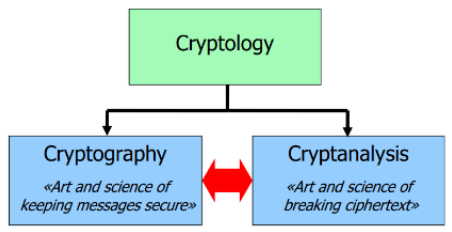
\includegraphics[width=0.6\linewidth]{its_goals.png}
\end{definition}

\begin{concept}{Business IT Risks}
\begin{itemize}
    \item Data loss
    \item System outage
    \item Espionage
    \item Sabotage
    \item Reputation loss
    \item Misuse of computing resources
    \item Violation of regulations
    \item Fraud
    \item Brand misuse
    \item Ransom demands
\end{itemize}
These risks can have significant financial, operational, and reputational impacts.
\end{concept}

\multend

\raggedcolumns

\subsubsection{Security Frameworks and Controls}

\mult{2}

\begin{concept}{Security Control Frameworks}
Security frameworks provide structured approaches to implementing security controls:
\begin{itemize}
    \item \textbf{CIS Controls} - Prioritized set of actions to protect organizations
    \item Controls are typically organized in implementation groups based on difficulty and impact
    \item Focus on preventing the most common attack vectors first
\end{itemize}
\end{concept}

\begin{definition}{Types of Security Measures}
Security measures can be categorized based on their focus:
\begin{itemize}
    \item \textbf{Preventive} - Block threats before they occur (firewalls, access controls)
    \item \textbf{Detective} - Identify when a breach has occurred (IDS, audit logs)
    \item \textbf{Corrective} - Mitigate damage after an incident (backups, incident response)
\end{itemize}
\end{definition}

\multend

\subsubsection{Disaster Recovery}



\begin{concept}{Business Continuity Management}
Disaster recovery and business continuity planning are essential for maintaining availability:
\begin{itemize}
    \item \textbf{Recovery Plan} - Detailed procedures for recovering from incidents
    \item \textbf{Recovery Tests} - Regular testing of recovery procedures
    \item \textbf{Redundancy} - Duplicate systems, power supplies, and network connections
    \item \textbf{Offline backups} - Protection against ransomware and other threats
\end{itemize}
\end{concept}

\begin{KR}{Disaster Recovery Planning}
\paragraph{Initial Assessment}
\begin{itemize}
    \item Identify critical systems and data
    \item Determine acceptable recovery time objectives (RTO)
    \item Determine acceptable recovery point objectives (RPO)
\end{itemize}

\paragraph{Plan Development}
\begin{itemize}
    \item Document recovery procedures
    \item Assign roles and responsibilities
    \item Include contact details for all relevant parties
    \item Develop technical instructions for restoration
\end{itemize}

\paragraph{Testing}
\begin{itemize}
    \item Conduct regular theoretical dry runs
    \item Perform practical tests (e.g., server shutdown, data restoration)
    \item Update procedures based on test results
\end{itemize}

\paragraph{Regular Review}
\begin{itemize}
    \item Review and update plans regularly
    \item Consider changes in infrastructure, personnel, and threats
\end{itemize}
\end{KR}

\begin{example}
A medium-sized company implements a disaster recovery plan for their customer database. They define an RTO of 4 hours and an RPO of 15 minutes, meaning they need to restore service within 4 hours with no more than 15 minutes of data loss. To achieve this, they implement a combination of hourly differential backups with continuous transaction log shipping to a standby site. Regular recovery tests are scheduled quarterly to ensure the plan remains effective.
\end{example}

\mult{2}


\begin{concept}{Problems - Overview}\\ and their impact on data availability
\paragraph{Physisch}
\textbf{unabsichtlich}
\begin{itemize}
    \item Naturkatastrophen
    \item Feuer
    \item Ausfall
    \item Kaffee auf Server
\end{itemize}

\textbf{absichtlich/bösartig}
\begin{itemize}
    \item Feuer
    \item Vandalismus
    \item Garantie läuft aus -> absichtlich langsamer
    \item Social Engineering
\end{itemize}

\paragraph{Virtuell}
\textbf{unabsichtlich}
\begin{itemize}
    \item Bitflip
    \item Config Fehler
    \item Bugs im SW
    \item Phishing klicken
\end{itemize}

\textbf{absichtlich/bösartig}
\begin{itemize}
    \item DDoS
    \item Malware
    \item Ransomware
    \item Phishing senden
    \item Trojaner
\end{itemize}
\end{concept}

\begin{theorem}{Countermeasures - Overview}

\textbf{Disaster Recovery}
    \begin{itemize}
        \item Offline backup solutions
        \item Restoring from images
    \end{itemize}

\textbf{Access Control}
    \begin{itemize}
        \item Restricted Access Rights
        \item Multi-Factor Authentication
        \item Firewalls
        \item Traffic Management Solutions
    \end{itemize}

\textbf{Physical Protection}
    \begin{itemize}
        \item Physical Access Control (locks, fences, etc.)
        \item Fire Protection (extinguishers, alarms, etc.)
        \item Monitoring (CCTV, Guards etc.)
    \end{itemize}

\textbf{Training Processes}
    \begin{itemize}
        \item Employee Training
        \item Four eyes principle
        \item Automation of routine processes
        \item Monitoring
        \item Preventive maintenance
    \end{itemize}

\textbf{Redundancy}
    \begin{itemize}
        \item Uninterruptable Power Supplies
        \item High Availability setups
        \item Load Balancing
        \item Redundant data center
        \item Redundant network connections
    \end{itemize}
\end{theorem}

\multend

\mult{2}

\begin{formula}{Recovery Plan and Test}

    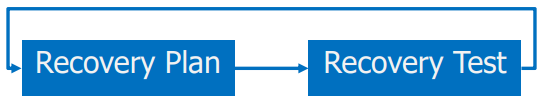
\includegraphics[width=0.7\linewidth]{recovery_plan_test.png}

    \textbf{Recovery Plan} - description of what to do if something goes wrong
    \begin{itemize}
        \item Roles and responsibilities
        \item Processes
        \item Contact details
        \item Technical instructions
    \end{itemize}

    \textbf{Recovery Test} - testing the recovery plan
    \begin{itemize}
        \item Theoretical dry run
        \item Practical tests
        \begin{itemize}
            \item turn off a server or DC
            \item restore data from backup
        \end{itemize}
    \end{itemize}
\end{formula}

\begin{concept}{Goals of IT Security}

Most measures in Information Security have one of the three following high-level goals:
\begin{itemize}
    \item Ensure data is confidential
    \item Ensure data is not corrupted
    \item Ensure data and systems are available
\end{itemize}

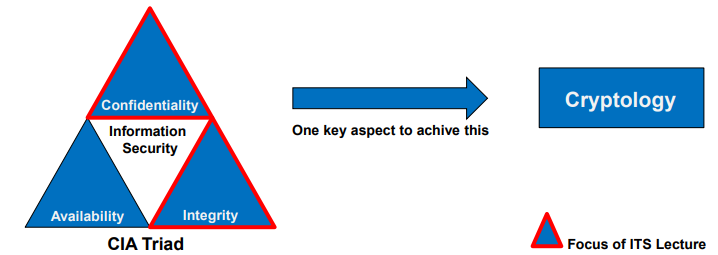
\includegraphics[width=\linewidth]{goals_of_IT_security.png}
\end{concept}

\multend

\raggedcolumns





	\section{Anforderungsanalyse}

\begin{definition}{Software Engineering}
\begin{itemize}
    \item \textbf{Disziplinen:} 
    Anforderungen, Architektur, Implementierung, Test und Wartung
    \item \textbf{Ziel:}  
    Strukturierte Prozesse für Qualität, Risiko- \& Fehlerminimierung
\end{itemize}
\end{definition} 

\subsection{Usability und User Experience}

\begin{concept}{Usability und User Experience} drei Säulen der Benutzererfahrung:
    \begin{itemize}
        \item \textbf{Usability (Gebrauchstauglichkeit):} \\ Grundlegende Nutzbarkeit des Systems
        \item \textbf{User Experience:} Usability + Desirability (Attraktivität)
        \item \textbf{Customer Experience:} \\ UX + Brand Experience (Markenwahrnehmung)
    \end{itemize}
    %todo: better resolution image
    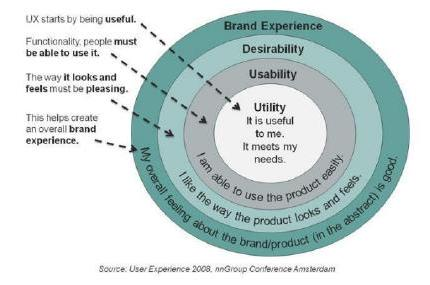
\includegraphics[width=0.6\linewidth]{images/2024_12_29_0d1d7b5551ea1b4b41bdg-02}
    
    \textbf{Wichtige Aspekte:}
    Benutzer und seine Ziele/Aufgaben, Kontext der Nutzung, Softwaresystem (inkl. UI)
\end{concept}

\begin{definition}{Usability-Dimensionen nach ISO 9241}
\begin{itemize}
    \item \textbf{Effektivität:}
    \begin{itemize}
        \item Der Benutzer kann alle Aufgaben vollständig erfüllen
        \item Gewünschte Genauigkeit wird erreicht
        \item Ziele werden im vorgegebenen Kontext erreicht
    \end{itemize}
    \end{itemize}

\begin{minipage}{0.5\linewidth}
    \begin{itemize}
    \item \textbf{Effizienz:} \\ Minimaler Aufwand für:
    \begin{itemize}
        \item Mentale Belastung
        \item Physische Anstrengung
        \item Zeitlicher Aufwand
        \item Ressourceneinsatz
    \end{itemize}
    \end{itemize}
\end{minipage}
\begin{minipage}{0.5\linewidth}
    \begin{itemize}
    \item \textbf{Zufriedenheit:}
    \begin{itemize}
        \item Minimum: Keine Verärgerung
        \item Standard: Zufriedenheit
        \item Optimal: Begeisterung
        \item Subjektive Nutzererfahrung
    \end{itemize}
\end{itemize}
\end{minipage}
\end{definition}

\begin{KR}{Usability-Evaluation durchführen}
\vspace{-2mm}\\
\begin{minipage}[t]{0.5\linewidth}
\begin{enumerate}[start=1]
    \item \textbf{Vorbereitung}
    \begin{itemize}
        \item Testziele definieren
        \item Testpersonen auswählen
        \item Testaufgaben erstellen
    \end{itemize}
    \item \textbf{Durchführung}
    \begin{itemize}
        \item Beobachtung der Nutzer
        \item Protokollierung von \\Problemen
        \item Zeitmessung der Aufgaben
    \end{itemize}
\end{enumerate}
\end{minipage}
\begin{minipage}[t]{0.5\linewidth}
\begin{enumerate}[start=3]
    \item \textbf{Auswertung}
    \begin{itemize}
        \item Probleme klassifizieren
        \item Schweregrad bestimmen
        \item Verbesserungen vorschlagen
    \end{itemize}
    
    \item \textbf{Dokumentation}
    \begin{itemize}
        \item Ergebnisse zusammenfassen
        \item Empfehlungen formulieren
        \item Maßnahmen priorisieren
    \end{itemize}
\end{enumerate}
\end{minipage}
\end{KR}

\begin{theorem}{ISO 9241-110: Usability-Anforderungen}

\begin{minipage}[t]{0.58\linewidth}
\begin{itemize}
    \item \textbf{Aufgabenangemessenheit:}
    \begin{itemize}
        \item Funktionalität unterstützt \\ Arbeitsaufgaben
        \item Keine unnötige Komplexität
    \end{itemize}
    
    \item \textbf{Selbstbeschreibungsfähigkeit:}
    \begin{itemize}
        \item Verständliche Benutzerführung
        \item Klare Statusanzeigen
    \end{itemize}
    
    \item \textbf{Steuerbarkeit:}
    \begin{itemize}
        \item Benutzer kontrolliert Ablauf
        \item Geschwindigkeit anpassbar
    \end{itemize}
    
    \item \textbf{Erwartungskonformität:}
    \begin{itemize}
        \item Konsistentes Verhalten
        \item Bekannte Konventionen
    \end{itemize}
\end{itemize}
\end{minipage}
\begin{minipage}[t]{0.4\linewidth}
\begin{itemize}    
    \item \textbf{Fehlertoleranz:}
    \begin{itemize}
        \item Fehler vermeiden
        \item Fehlerkorrektur \\ ermöglichen
    \end{itemize}
    
    \item \textbf{Individualisierbarkeit:}
    \begin{itemize}
        \item Anpassung an \\ Benutzergruppen
        \item Flexible Nutzung
    \end{itemize}
    
    \item \textbf{Lernförderlichkeit:}
    \begin{itemize}
        \item Einfacher Einstieg
        \item Unterstützung beim \\ Lernen
    \end{itemize}
\end{itemize}
\end{minipage}
\end{theorem}

\subsection{User-Centered Design (UCD)}

\begin{concept}{UCD Prozess}

\begin{minipage}{0.4\linewidth}
Ein iterativer Prozess zur nutzerzentrierten \\ Entwicklung, der die Bedürfnisse, Wünsche und Einschränkungen 
der Benutzer in jeder Phase des Design-Prozesses berücksichtigt.

\textbf{Hauptziele:}
\begin{itemize}
    \item Benutzerfreundlichkeit
    \item Effektive Nutzung
    \item Hohe Akzeptanz
\end{itemize}
\end{minipage}
\begin{minipage}{0.6\linewidth}
    \vspace{-5mm}
    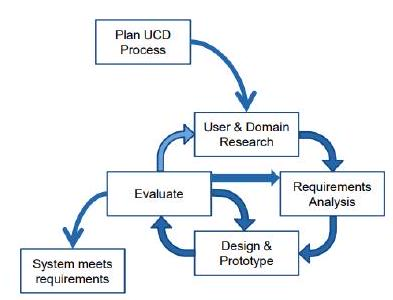
\includegraphics[width=\linewidth]{images/2024_12_29_0d1d7b5551ea1b4b41bdg-03}
\end{minipage}
\end{concept}

\begin{corollary}{Wichtige Artefakte}
\begin{itemize}
    \item Personas: Repräsentative Nutzerprofile
    \item Usage-Szenarien: Konkrete Anwendungsfälle
    \item Mentales Modell: Nutzerverständnis
    \item Domänenmodell: Fachliches Verständnis
    \item Service Blueprint: Geschäftsprozessmodell
    \item Stakeholder Map: Beteiligte und Betroffene
    \item UI-Artefakte: Skizzen, Wireframes, Designs
\end{itemize}
\end{corollary}

\begin{example2}{Stakeholder Map}\\
Zeigt die wichtigsten Stakeholder im Umfeld der Problemdomäne.\\
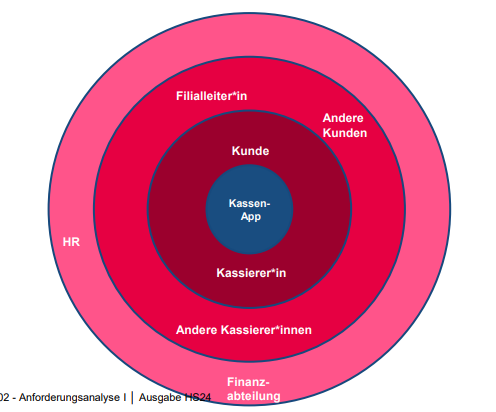
\includegraphics[width=0.8\linewidth]{images/stakeholdermap.png}
\end{example2}



\begin{theorem}{UCD Prozess-Phasen}\\
\textbf{1. User \& Domain Research} (see KR)

\textbf{2. Requirements Analysis} (see KR)

\begin{minipage}[t]{0.5\linewidth}
\textbf{3. Design \& Prototype}
\begin{itemize}
    \item Interaktionskonzept entwickeln
    \item Wireframes erstellen
    \item Prototypen bauen
    \item Design iterativ verbessern
\end{itemize}
\end{minipage}
\begin{minipage}[t]{0.5\linewidth}
\textbf{4. Evaluate}
\begin{itemize}
    \item Mit Benutzern testen
    \item Feedback sammeln
    \item Probleme identifizieren
    \item Verbesserungen einarbeiten
\end{itemize}
\end{minipage}
\end{theorem}

\begin{KR}{User \& Domain Research}
\begin{enumerate}
    \item \textbf{Zielgruppe identifizieren}
    \begin{itemize}
        \item Wer sind die Benutzer?
        \item Was sind ihre Aufgaben/Ziele?
        \item Wie sieht ihre Arbeitsumgebung aus?
        \item Welche Sprache/Begriffe verwenden sie?
    \end{itemize}
\end{enumerate}

\begin{minipage}[t]{0.5\linewidth}
\begin{enumerate}[start=2]
    \item \textbf{Daten sammeln durch}
    \begin{itemize}
        \item Contextual Inquiry
        \item Interviews
        \item Beobachtung
        \item Fokusgruppen
        \item Nutzungsauswertung
    \end{itemize}
\end{enumerate}
\end{minipage}
\begin{minipage}[t]{0.5\linewidth}
\begin{enumerate}[start=3]
    \item \textbf{Ergebnisse dokumentieren in}
    \begin{itemize}
        \item Personas
        \item Usage-Szenarien
        \item Mentales Modell
    \end{itemize}
\end{enumerate}
\end{minipage}
\end{KR}

\begin{KR}{UCD Artefakte erstellen}

\begin{minipage}[t]{0.45\linewidth}
\textbf{1. Personas}
\begin{itemize}
    \item Daten aus User Research\\ sammeln
    \item Gemeinsame Merkmale \\identifizieren
    \item Repräsentative Person \\definieren
    \item Details ausarbeiten:
    \begin{itemize}
        \item Demografische Daten
        \item Ziele und Motivation
        \item Fähigkeiten/Kenntnisse
        \item Frustrationspunkte
    \end{itemize}
\end{itemize}
\end{minipage}
\begin{minipage}[t]{0.5\linewidth}
\textbf{2. Usage-Szenarien}
\begin{itemize}
    \item Kontext beschreiben
    \item Akteure identifizieren
    \item Ablauf definieren
    \item Probleme/Lösungen darstellen
\end{itemize}

\textbf{3. Mentales Modell}
\begin{itemize}
    \item Nutzerverständnis\\ dokumentieren
    \item Konzepte und Beziehungen \\visualisieren
    \item Mit Fachmodell abgleichen
\end{itemize}
\end{minipage}
\end{KR}

\begin{example2}{Usage-Szenario: Online-Banking}\\
\textbf{Kontext:} Sarah möchte eine Überweisung tätigen

\textbf{Aktuelles Szenario:}
Sarah loggt sich in ihr Online-Banking ein. Sie sucht nach der letzten Überweisung an ihren Vermieter, um die Kontodetails zu finden. Nach mehreren Klicks findet sie die Information und kopiert die IBAN. Sie öffnet das Überweisungsformular und fügt die Daten ein. Beim Absenden erscheint eine Fehlermeldung, weil sie vergessen hat, den Verwendungszweck einzutragen.

\textbf{Probleme:}
\begin{itemize}
    \item Umständliche Suche nach Kontodetails
    \item Fehleranfällige manuelle Dateneingabe
    \item Späte Validierung der Eingaben
\end{itemize}

\textbf{Verbessertes Szenario:}
Sarah wählt aus einer Liste ihrer häufigen Empfänger ihren Vermieter aus. Das System füllt automatisch alle bekannten Daten ein. Fehlende Pflichtfelder sind deutlich markiert. Sarah ergänzt den Verwendungszweck und sendet die Überweisung ab.
\end{example2}

\begin{remark}
    Weitere Beispiele z.B. Persona erstellen auf nächster Seite
\end{remark}

\begin{example2}{Persona erstellen}\\
\textbf{Aufgabe:} Erstellen Sie eine Persona für ein Online-Banking-System.

\textbf{Lösung:} 
\textbf{Sarah Schmidt, 34, Projektmanagerin}
\begin{itemize}
    \item \textbf{Hintergrund:}
    \begin{itemize}
        \item Arbeitet Vollzeit in IT-Firma
        \item Technik-affin, aber keine Expertin
        \item Nutzt Smartphone für die meisten Aufgaben
    \end{itemize}
    \item \textbf{Ziele:}
    \begin{itemize}
        \item Schnelle Überweisungen zwischen Konten
        \item Überblick über Ausgaben
        \item Sichere Authentifizierung
    \end{itemize}
    \item \textbf{Frustrationen:}
    \begin{itemize}
        \item Komplexe Menüführung
        \item Lange Ladezeiten
        \item Mehrfache Login-Prozesse
    \end{itemize}
\end{itemize}
\end{example2}

\begin{example2}{Persona für E-Learning-System}\\
\textbf{Thomas Weber, 19, Informatik-Student}

\textbf{Hintergrund:}
\begin{itemize}
    \item Erstsemester-Student
    \item Arbeitet nebenbei 10h/Woche
    \item Pendelt zur Universität (1h pro Weg)
\end{itemize}

\textbf{Technische Fähigkeiten:}
\begin{itemize}
    \item Versiert im Umgang mit Computern
    \item Nutzt hauptsächlich Smartphone für Online-Aktivitäten
    \item Kennt gängige Learning-Management-Systeme
\end{itemize}

\textbf{Ziele:}
\begin{itemize}
    \item Effizientes Lernen trotz Zeitdruck
    \item Flexible Zugriffsmöglichkeiten auf Lernmaterialien
    \item Gute Prüfungsvorbereitung
\end{itemize}

\textbf{Frustrationen:}
\begin{itemize}
    \item Unübersichtliche Kursstrukturen
    \item Fehlende Mobile-Optimierung
    \item Schwierige Navigation zwischen Materialien
\end{itemize}
\end{example2}

\subsection{Requirements Engineering}

\begin{definition}{Requirements (Anforderungen)}
\begin{itemize}
    \item Leistungsfähigkeiten oder Eigenschaften
    \item Explizit oder implizit
    \item Müssen mit allen Stakeholdern erarbeitet werden
    \item Entwickeln sich während des Projekts
\end{itemize}
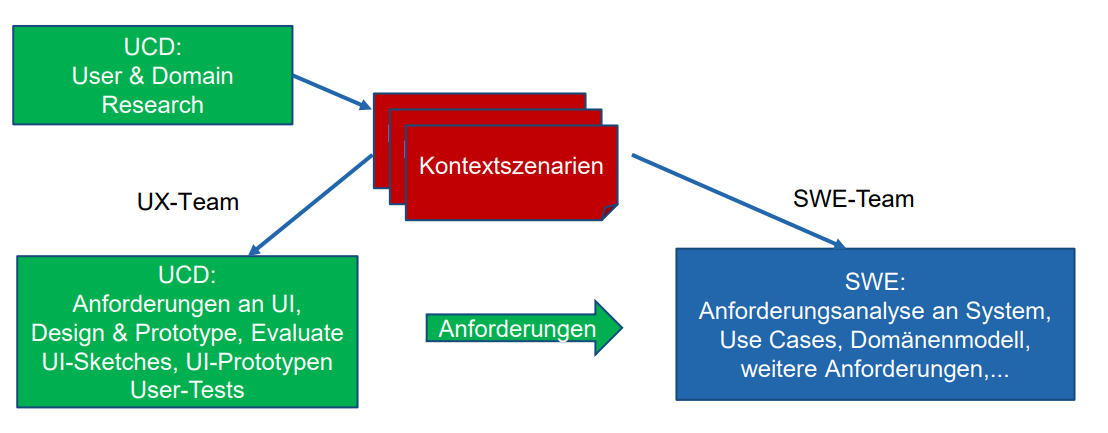
\includegraphics[width=\linewidth]{images/user_anforderungen.png}

\textbf{Charakteristiken:}
\begin{itemize}
    \item Können explizit oder implizit sein
    \item Sind fast nie im Vorneherein vollständig bekannt
    \item Müssen mit allen Stakeholdern erarbeitet werden
    \item Entwickeln sich während des Projekts
    \item Müssen verifizierbar und messbar sein
\end{itemize}

\textbf{Herkunft:}
\begin{itemize}
    \item Benutzer (Ziele, Bedürfnisse, Kontext)
    \item Weitere Stakeholder (Management, IT, etc.)
    \item Regulatorien, Gesetze, Normen
\end{itemize}
\end{definition}





\begin{concept}{Arten von Anforderungen}\\
\textbf{Funktionale Anforderungen:}
\begin{itemize}
    \item Beschreiben, WAS das System tun soll
    \item Werden in Use Cases dokumentiert
    \item Müssen konkret und testbar sein
\end{itemize}

\textbf{Nicht-funktionale Anforderungen (ISO 25010):}
\begin{itemize}
    \item Performance Efficiency
    \begin{itemize}
        \item Time Behaviour
        \item Resource Utilization
        \item Capacity
    \end{itemize}
    \item Compatibility
    \begin{itemize}
        \item Co-existence
        \item Interoperability
    \end{itemize}
    \item Usability (siehe oben)
    \item Reliability
    \begin{itemize}
        \item Maturity
        \item Availability
        \item Fault Tolerance
        \item Recoverability
    \end{itemize}
    \item Security
    \item Maintainability
    \item Portability
\end{itemize}

\textbf{Randbedingungen:}
\begin{itemize}
    \item Technische Einschränkungen
    \item Rechtliche Vorgaben
    \item Budgetäre Grenzen
    \item Zeitliche Limitationen
\end{itemize}
\end{concept}

\begin{KR}{Requirements Analysis}
    \begin{itemize}
        \item Benutzeranforderungen ableiten
        \item Kontextszenarien erstellen
        \item UI-Skizzen entwickeln
        \item Use Cases definieren
    \end{itemize}
    \vspace{2mm}

    \begin{minipage}[t]{0.45\linewidth}
    \textbf{Stakeholder identifizieren}
    \begin{itemize}
        \item Benutzer
        \item Auftraggeber
        \item Weitere Interessengruppen
    \end{itemize}
    
    \textbf{Anforderungsquellen \\ analysieren}
    \begin{itemize}
        \item Interviews und Workshops
        \item Existierende Dokumente
        \item Beobachtung der \\Arbeitsabläufe
    \end{itemize}
    \end{minipage}
    \begin{minipage}[t]{0.55\linewidth}    
    \textbf{Anforderungen dokumentieren}
    \begin{itemize}
        \item Funktionale Anforderungen \\ (Use Cases)
        \item Nicht-funktionale Anforderungen
        \item Randbedingungen
    \end{itemize}
    
    \textbf{Anforderungen validieren}
    \begin{itemize}
        \item Review mit Stakeholdern
        \item Priorisierung
        \item Machbarkeitsanalyse
    \end{itemize}
    \end{minipage}
\end{KR}

\begin{example2}{Anforderungsanalyse: Onlineshop}\\
\textbf{Ausgangssituation:}
Ein traditioneller Buchladen möchte einen Onlineshop entwickeln.

\textbf{Funktionale Anforderungen:}
\begin{itemize}
    \item Produktkatalog durchsuchen
    \item Warenkorb verwalten
    \item Bestellung aufgeben
    \item Kundenkonto verwalten
\end{itemize}

\textbf{Nicht-funktionale Anforderungen:}
\begin{itemize}
    \item Performance:
    \begin{itemize}
        \item Seitenaufbau < 2 Sekunden
        \item Suche < 1 Sekunde
    \end{itemize}
    \item Sicherheit:
    \begin{itemize}
        \item HTTPS-Verschlüsselung
        \item Zwei-Faktor-Authentifizierung
    \end{itemize}
    \item Usability:
    \begin{itemize}
        \item Responsive Design
        \item Max. 3 Klicks zur Bestellung
    \end{itemize}
\end{itemize}

\textbf{Randbedingungen:}
\begin{itemize}
    \item DSGVO-Konformität
    \item Integration mit bestehendem ERP
    \item Budget: 100.000 EUR
    \item Launch in 6 Monaten
\end{itemize}
\end{example2}

\columnbreak



\subsection{Use Cases}

\begin{definition}{Use Case (Anwendungsfall)}\\
Ein Use Case beschreibt eine konkrete Interaktion zwischen Akteur und System mit folgenden Eigenschaften:

\textbf{Grundprinzipien:}
\begin{itemize}
    \item Aus Sicht des Akteurs beschrieben
    \item Aktiv formuliert (Verb + Objekt)
    \item Konkreter Nutzen für Akteur
    \item Mehr als eine einzelne Interaktion
    \item Essentieller Stil (Logik statt Implementierung)
\end{itemize}

\textbf{Qualitätskriterien:}
\begin{itemize}
    \item Boss-Test: Sinnvolle Arbeitseinheit
    \item EBP-Test: Elementary Business Process
    \item Size-Test: Mehrere Interaktionen
\end{itemize}
\end{definition}

\begin{KR}{Use Case Erstellung}\\
Schritte zur Erstellung eines vollständigen Use Cases:
\begin{enumerate}
    \item \textbf{Identifikation:} siehe \textcolor{green}{\textbf{Use Case Identifikation}}
    \item \textbf{Dokumentation:}
    \begin{itemize}
        \item Brief/Casual für erste Analyse
        \item Fully-dressed für wichtige Use Cases
        \item Standardablauf und Erweiterungen
    \end{itemize}
    \item \textbf{Review:}
    \begin{itemize}
        \item Mit Stakeholdern abstimmen
        \item Auf Vollständigkeit prüfen
        \item Konsistenz sicherstellen
    \end{itemize}
\end{enumerate}
\end{KR}

\begin{theorem}{Use Case Identifikation}
\begin{enumerate}
    \item \textbf{Systemgrenzen definieren}
    \begin{itemize}
        \item Was gehört zum System?
        \item Was ist externe Umgebung?
    \end{itemize}
    \item \textbf{Akteure identifizieren}
    \item \textbf{Ziele ermitteln}
    \begin{itemize}
        \item Geschäftsziele
        \item Benutzerziele
        \item Systemziele
    \end{itemize}
\end{enumerate}
\end{theorem}

\begin{corollary}{Akteure in Use Cases}
\begin{itemize}
    \item \textbf{Primärakteur:} Initiiert den Use Case, erhält Hauptnutzen
    \item \textbf{Unterstützender Akteur:} Hilft bei der Durchführung
    \item \textbf{Offstage-Akteur:} Indirekt beteiligter Stakeholder
\end{itemize}
\end{corollary}

\begin{concept}{Use Case Beziehungen}\\
\textbf{Include-Beziehung:}
\begin{itemize}
    \item Ein UC schließt einen anderen UC ein
    \item Wiederverwendung von Funktionalität
    \item Obligatorische Beziehung
\end{itemize}

\textbf{Extend-Beziehung:}
\begin{itemize}
    \item Optionale Erweiterung eines UC
    \item Unter bestimmten Bedingungen
    \item Ursprünglicher UC bleibt unverändert
\end{itemize}

\textbf{Generalisierung:}
\begin{itemize}
    \item Spezialisierung von Akteuren/UCs
    \item Vererbung von Eigenschaften
    \item "ist-ein"-Beziehung
\end{itemize}
\end{concept}

\begin{concept}{Use Case Granularität}
\begin{enumerate}
    \item \textbf{Brief Use Case}
    \begin{itemize}
        \item Kurze Zusammenfassung
        \item Hauptablauf skizzieren
        \item Keine Details zu Varianten
    \end{itemize}
    \item \textbf{Casual Use Case}
    \begin{itemize}
        \item Mehrere Absätze
        \item Hauptvarianten beschreiben
        \item Informeller Stil
    \end{itemize}
    \item \textbf{Fully-dressed Use Case}
    \begin{itemize}
        \item Vollständige Struktur
        \item Alle Varianten
        \item Vor- und Nachbedingungen
        \item Garantien definieren
    \end{itemize}
\end{enumerate}
\end{concept}

\begin{KR}{Fully-dressed Use Case erstellen}

\begin{minipage}[t]{0.55\linewidth}
\textbf{1. Grundinformationen}
\begin{itemize}
    \item Aussagekräftiger Name (aktiv)
    \item Umfang (Scope)
    \item Ebene (Level)
    \item Primärakteur
\end{itemize}

\textbf{2. Stakeholder und Interessen}
\begin{itemize}
    \item Alle beteiligten Parteien
    \item Deren spezifische Interessen
\end{itemize}

\textbf{3. Vor- und Nachbedingungen}
\begin{itemize}
    \item Was muss vorher erfüllt sein?
    \item Was ist nachher garantiert?
\end{itemize}
\end{minipage}
\begin{minipage}[t]{0.45\linewidth}
\textbf{4. Standardablauf}
\begin{itemize}
    \item Nummerierte Schritte
    \item Akteur-System-Interaktion
    \item Klare Erfolgskriterien
\end{itemize}

\textbf{5. Erweiterungen}
\begin{itemize}
    \item Alternative Abläufe
    \item Fehlerszenarien
    \item Verzweigungen
\end{itemize}
\end{minipage}
\end{KR}

\begin{example2}{Brief Use Case}
\textbf{Verkauf abwickeln}

Kunde kommt mit Waren zur Kasse. Kassier erfasst alle Produkte. System berechnet Gesamtbetrag. Kassier nimmt Zahlung entgegen und gibt ggf. Wechselgeld. System druckt Beleg.
\end{example2}

%TODO: Add casual use case?

\begin{example2}{Casual Use Case}
\textbf{UC: Verkauf abwickeln}
Der Umfang des Use Cases ist das Kassensystem. Der Primärakteur ist der Kassier. 
Der Stakeholder ist der Kunde, der eine schnelle Abwicklung wünscht, und das Geschäft, das eine korrekte Abrechnung benötigt. 
Die Vorbedingung ist, dass die Kasse geöffnet ist.
\vspace{2mm}\\
Der Standardablauf ist wie folgt:
Kassier startet neuen Verkauf und System initialisiert neue Transaktion. Kassier erfasst Produkte und System zeigt Zwischensumme. 
Kassier schliesst Verkauf ab und System zeigt Gesamtbetrag. Kunde bezahlt und System druckt Beleg.
\end{example2}


\begin{example2}{Fully-dressed Use Case}
\textbf{UC: Verkauf abwickeln}
\begin{itemize}
    \item \textbf{Umfang:} Kassensystem
    \item \textbf{Primärakteur:} Kassier
    \item \textbf{Stakeholder:} Kunde (schnelle Abwicklung), Geschäft (korrekte Abrechnung)
    \item \textbf{Vorbedingung:} Kasse ist geöffnet
    \item \textbf{Standardablauf:}
    \begin{enumerate}
        \item Kassier startet neuen Verkauf
        \item System initialisiert neue Transaktion
        \item Kassier erfasst Produkte
        \item System zeigt Zwischensumme
        \item Kassier schliesst Verkauf ab
        \item System zeigt Gesamtbetrag
        \item Kunde bezahlt
        \item System druckt Beleg
    \end{enumerate}
\end{itemize}
\end{example2}

\begin{example2}{Fully-dressed Use Case}
\textbf{Aufgabe:} Erstellen Sie einen fully-dressed Use Case für ein Online-Bibliothekssystem. Fokus: "Buch ausleihen"

\textbf{Lösung:}
\begin{itemize}
    \item \textbf{Umfang:} Online-Bibliothekssystem
    \item \textbf{Primärakteur:} Bibliotheksnutzer
    \item \textbf{Stakeholder:} 
    \begin{itemize}
        \item Bibliotheksnutzer: Möchte Buch einfach ausleihen
        \item Bibliothek: Korrekte Erfassung der Ausleihe
    \end{itemize}
    \item \textbf{Vorbedingung:} Nutzer ist eingeloggt
    \item \textbf{Standardablauf:}
    \begin{enumerate}
        \item Nutzer sucht Buch
        \item System zeigt Verfügbarkeit
        \item Nutzer wählt Ausleihe
        \item System prüft Ausleihberechtigung
        \item System registriert Ausleihe
        \item System zeigt Bestätigung
    \end{enumerate}
    \item \textbf{Erweiterungen:}
    \begin{itemize}
        \item 2a: Buch nicht verfügbar
        \item 4a: Keine Ausleihberechtigung
    \end{itemize}
\end{itemize}
\end{example2}

\begin{example2}{Typische Prüfungsaufgabe: Use Case Analyse}\\
\textbf{Aufgabe:} Analysieren Sie den folgenden Use Case und identifizieren Sie mögliche Probleme:

\textbf{Use Case:} "Der Benutzer loggt sich ein und das System zeigt die Startseite. Er klickt auf den Button und die Daten werden in der Datenbank gespeichert."

\textbf{Probleme:}
\begin{itemize}
    \item Zu technisch/implementierungsnah
    \item Fehlende Akteurperspektive
    \item Unklarer Nutzen/Ziel
    \item Fehlende Alternativszenarien
    \item Keine Fehlerbehandlung
\end{itemize}

\textbf{Verbesserter Use Case:}
"Der Kunde möchte seine Bestelldaten speichern. Er bestätigt die Eingaben und erhält eine Bestätigung über die erfolgreiche Speicherung."
\end{example2}

\begin{example2}{Prüfungsaufgabe: Use Case Analyse}\\
\textbf{Aufgabe:} Analysieren Sie folgenden Use Case und verbessern Sie ihn.

\textbf{Ursprünglicher Use Case:}
"Der User loggt sich ein. Das System überprüft seine Credentials in der Datenbank. 
Bei erfolgreicher Validierung wird die Startseite angezeigt. Der User klickt auf 'Profil bearbeiten' 
und das System speichert die Änderungen in der Datenbank."

\textbf{Probleme:}
\begin{itemize}
    \item Technische Implementierungsdetails
    \item Fehlende Akteurperspektive
    \item Keine Alternativen/Fehlerbehandlung
    \item Unklarer Nutzen/Ziel
\end{itemize}

\textbf{Verbesserter Use Case:}
"Profilinformationen aktualisieren"
\begin{itemize}
    \item \textbf{Primärakteur:} Registrierter Benutzer
    \item \textbf{Vorbedingung:} Benutzer ist authentifiziert
    \item \textbf{Standardablauf:}
    \begin{enumerate}
        \item Benutzer wählt Profilbearbeitung
        \item System zeigt aktuelle Profildaten
        \item Benutzer ändert gewünschte Informationen
        \item System prüft Änderungen
        \item System bestätigt erfolgreiche Aktualisierung
    \end{enumerate}
    \item \textbf{Erweiterungen:}
    \begin{itemize}
        \item 4a: Ungültige Eingaben
        \item 4b: Verbindungsfehler
    \end{itemize}
\end{itemize}
\end{example2}



\columnbreak

\subsection{Use Case Diagrams}

\begin{definition}{Use Case Diagramm}\\
    Zeigt:
    \begin{itemize}
        \item Systemabgrenzung
        \item Akteure: Primärakteure initiieren UCs, unterstützende sind beteiligt
    \end{itemize}
    Liste der Anwendungsfälle:
    \begin{itemize}
        \item Process Sale
        \item Cash in
        \item Cash out
        \item Handle Returns
        \item Manage Users
    \end{itemize}
    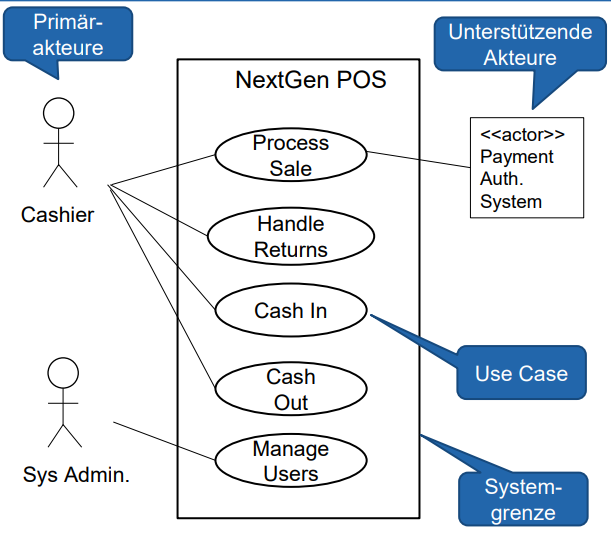
\includegraphics[width=\linewidth]{uc_diagram.png}
\end{definition}

\begin{concept}
    {Zusätzliche Beziehungen im UC-Diagramm}

    <<include>>
    \begin{itemize}
        \item Ein UC kann ein anderes UC inkludieren
        \item Wiederverwendung von Funktionalität
        \item Obligatorische Beziehung
        \item UC „Process Sale" inkludiert UC „Handle Cash Payment"
        \item UC „Process Sale" inkludiert UC „Handle TWINT Payment"
        \item Sie sind hier aber keine eigenständigen UCs (keine Verbindung zu Akteuren)
        \item Included UCs können auch selbständige UC sein.
    \end{itemize}
    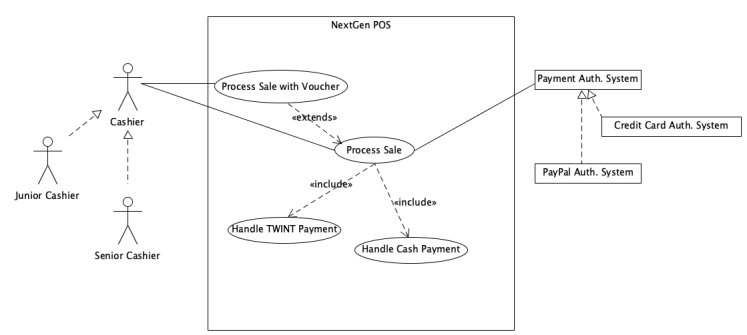
\includegraphics[width=\linewidth]{includebez.png}

    <<extends>>
    \begin{itemize}
        \item Eigenständiger UC, der eine Erweiterung eines anderen darstellt, und
        \item ursprünglicher UC nicht verändert werden soll
        \item Sonst besser als Erweiterung im UC-Text einfügen
        \item Akteur-Generalisierung
        \item Um Akteure zusammenzufassen
        \item Kann als „ist-ein"-Beziehung modelliert werden
    \end{itemize}
    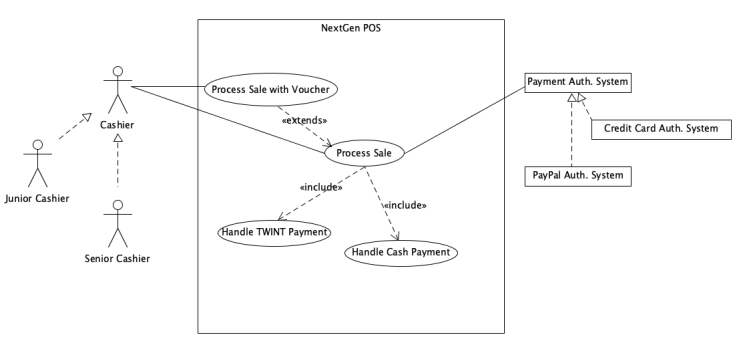
\includegraphics[width=\linewidth]{extendbez.png}
\end{concept}

\pagebreak

\subsection{System Sequence Diagrams}

\begin{definition}{Systemsequenzdiagramm (SSD)}\\
Formalisierte Darstellung der System-Interaktionen:

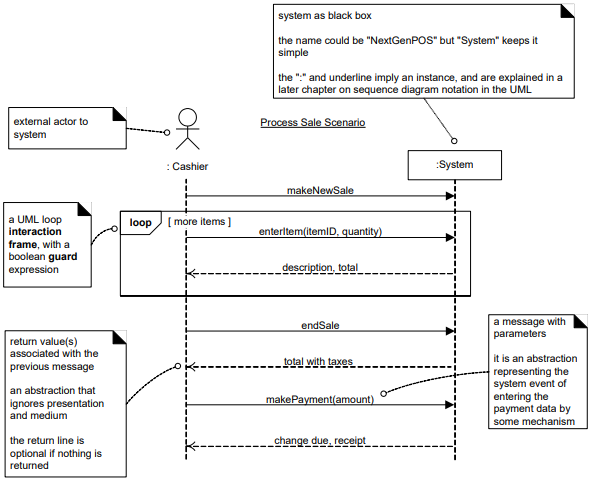
\includegraphics[width=\linewidth]{ssed.png}
\end{definition}

\begin{concept}{System Sequence Diagram}\\
Ein SSD visualisiert die Interaktion zwischen Akteur und System auf einer höheren Abstraktionsebene:

\textbf{Hauptmerkmale:}
\begin{itemize}
    \item Zeigt Input/Output-Events
    \item Identifiziert Systemoperationen
    \item Bildet Basis für API-Design
    \item Abstrahiert von UI-Details
\end{itemize}

\textbf{Notationselemente:}
\begin{itemize}
    \item Akteur und System als Lebenslinien
    \item Methodenaufrufe als durchgezogene Pfeile
    \item Rückgabewerte als gestrichelte Pfeile
    \item Parameter für benötigte Informationen
\end{itemize}
\end{concept}

\begin{KR}{System Sequence Diagram erstellen}\\
\textbf{1. Vorbereitung}
\begin{itemize}
    \item Use Case als Grundlage wählen
    \item Standardablauf identifizieren
    \item Akteur und System festlegen
\end{itemize}

\textbf{2. Methodenaufrufe definieren}
\begin{itemize}
    \item Aussagekräftige Namen wählen
    \item Notwendige Parameter bestimmen
    \item Rückgabewerte festlegen
\end{itemize}

\textbf{3. Zeitliche Abfolge}
\begin{itemize}
    \item Sequenz der Aufrufe modellieren
    \item Abhängigkeiten beachten
    \item Kontrollstrukturen einbauen (alt, loop, etc.)
\end{itemize}

\textbf{4. Externe Systeme}
\begin{itemize}
    \item Bei Bedarf weitere Akteure einbinden
    \item Schnittstellen definieren
    \item Kommunikationsfluss darstellen
\end{itemize}
\end{KR}

\begin{KR}{Systemoperationen definieren}\\
\textbf{Namenskonventionen:}
\begin{itemize}
    \item Verben für Aktionen
    \item Substantive für Entitäten
    \item Präzise, aber nicht technisch
\end{itemize}

\textbf{Parameter:}
\begin{itemize}
    \item Nur notwendige Information
    \item Domänenorientierte Typen
    \item Sinnvolle Standardwerte
\end{itemize}

\textbf{Rückgabewerte:}
\begin{itemize}
    \item Eindeutige Bestätigungen
    \item Relevante Geschäftsobjekte
    \item Fehlerindikationen
\end{itemize}

\textbf{Beispiele guter Operationen:}
\begin{lstlisting}[language=Java, style=base]
// Gut - klar und domaenenorientiert
createOrder(customer: CustomerId): OrderId
addOrderItem(orderId: OrderId, 
            product: ProductId, 
            quantity: int)

// Schlecht - zu technisch/implementierungsnah
insertIntoOrderTable(customerData: Map)
updateOrderItemList(items: ArrayList)
\end{lstlisting}
\end{KR}

\begin{KR}{Operation Contracts}\\
Ein Contract definiert die Vor- und Nachbedingungen einer Systemoperation:

\textbf{1. Struktur}
\begin{itemize}
    \item Name und Parameter
    \item Querverweis zum Use Case
    \item Vorbedingungen
    \item Nachbedingungen
\end{itemize}

\textbf{2. Vorbedingungen}
\begin{itemize}
    \item Systemzustand vor Aufruf
    \item Notwendige Initialisierungen
    \item Gültige Parameter
\end{itemize}

\textbf{3. Nachbedingungen}
\begin{itemize}
    \item Erstellte/gelöschte Instanzen
    \item Geänderte Attribute
    \item Neue/gelöschte Assoziationen
\end{itemize}
\end{KR}

\begin{remark}
    Wann Operation Contracts?

    - Nur wenn aus einem Anwendungsfall nicht klar wird, was die Systemoperation genau machen muss
    
    - Meist nur bei sehr komplizierten Operationen und/oder
    
    - Wenn Entwicklung der Systemoperation ausgelagert wird (anderes Team, externe Entwickler)
    
    - Erst gegen Ende des Meilensteins Lösungsarchitektur oder kurz vor Start des Designs der Systemoperation
\end{remark}

\begin{example2}{Contract für enterItem()}\\
\textbf{Operation:} enterItem(itemId: ItemID, quantity: int)

\textbf{Querverweis:} UC "Process Sale"

\textbf{Vorbedingungen:}
\begin{itemize}
    \item Verkauf ist gestartet
    \item ItemID existiert im System
\end{itemize}

\textbf{Nachbedingungen:}
\begin{itemize}
    \item SalesLineItem-Instanz wurde erstellt
    \item Verknüpfung mit aktueller Sale-Instanz
    \item quantity wurde gesetzt
    \item Verknüpfung mit ProductDescription
\end{itemize}
\end{example2}

\begin{example2}{SSD für Interaktion zwischen 2 Systemen}\\
    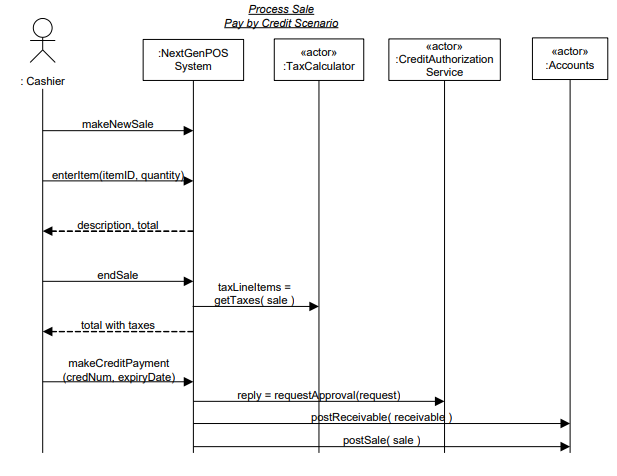
\includegraphics[width=\linewidth]{ssdzweisysteme.png}
\end{example2}


\begin{example2}{SSD Übungsaufgabe}\\
\textbf{Aufgabe:} Erstellen Sie ein Systemsequenzdiagramm für den Use Case 'Geld abheben' an einem Bankautomaten.

\textbf{Wichtige Aspekte:}
\begin{itemize}
    \item Kartenvalidierung
    \item PIN-Eingabe
    \item Betragseingabe
    \item Kontostandsprüfung
    \item Geldausgabe
    \item Belegdruck
\end{itemize}

\textbf{Essentielle Systemoperationen:}
\begin{itemize}
    \item validateCard(cardNumber)
    \item checkPIN(pin)
    \item withdrawMoney(amount)
    \item printReceipt()
\end{itemize}

\textbf{Sequenzdiagramm:} %TODO: add SSD graphic
\textcolor{pink}{\textbf{TO BE ADDED}}
\end{example2}


\begin{example2}{SSD: Online-Banking Überweisung}\\
\textbf{Use Case:} Überweisung durchführen

\textbf{Systemoperationen:}
\begin{lstlisting}[language=Java, style=base]
// Kontostand pruefen
checkBalance(): Money

// Ueberweisung initiieren
initiateTransfer(recipient: String, 
                iban: String, 
                amount: Money, 
                purpose: String): TransferId

// TAN anfordern
requestTAN(transferId: TransferId): void

// Ueberweisung bestaetigen
confirmTransfer(transferId: TransferId, 
               tan: String): Boolean
\end{lstlisting}

\textbf{Wichtige Aspekte:}
\begin{itemize}
    \item Validierung vor Ausführung
    \item Zweistufige Bestätigung
    \item Klare Rückmeldungen
    \item Fehlerbehandlung
\end{itemize}

\textbf{Sequenzdiagramm:} %TODO: add SSD graphic
\textcolor{pink}{\textbf{TO BE ADDED}}
\end{example2}


\begin{example2}{SSD: Typische Prüfungsaufgabe}\\
\textbf{Aufgabe:} Erstellen Sie ein SSD für den Use Case "Produkt bestellen" in einem Webshop.

\textbf{Analyse:}
\begin{itemize}
    \item Identifiziere Hauptaktionen:
    \begin{itemize}
        \item Warenkorb verwalten
        \item Bestellung aufgeben
        \item Zahlung durchführen
    \end{itemize}
    
    \item Definiere Systemoperationen:
    \begin{itemize}
        \item addToCart(productId, quantity)
        \item showCart(): CartContents
        \item checkout(shippingAddress, paymentMethod)
        \item confirmOrder(): OrderId
    \end{itemize}
    
    \item Berücksichtige Rückgabewerte:
    \begin{itemize}
        \item Bestätigungen
        \item Zwischensummen
        \item Fehlermeldungen
    \end{itemize}
\end{itemize}

\textbf{Sequenzdiagramm:} %TODO: add SSD graphic
\textcolor{pink}{\textbf{TO BE ADDED}}
\end{example2}


\begin{example2}{SSD: Integration mit externen Systemen}\\
\textbf{Use Case:} Kreditkartenzahlung durchführen

\textbf{Beteiligte Systeme:}
\begin{itemize}
    \item Verkaufssystem (SuD)
    \item Kreditkarten-Autorisierungssystem
    \item Buchhaltungssystem
\end{itemize}

\textbf{Systemoperationen:}
\begin{lstlisting}[language=Java, style=base]
// Request credit card approval
requestApproval(cardNum: String, 
               expiryDate: Date, 
               amount: Money): Boolean

// Post transaction to accounting
postTransaction(transactionData: TransactionData)
\end{lstlisting}

\textbf{Wichtige Aspekte:}
\begin{itemize}
    \item Asynchrone Kommunikation
    \item Fehlerbehandlung über mehrere Systeme
    \item Transaktionsmanagement
    \item Logging und Nachvollziehbarkeit
\end{itemize}

\textbf{Sequenzdiagramm:} %TODO: add SSD graphic
\textcolor{pink}{\textbf{TO BE ADDED}}
\end{example2}
	%\input{02_domänenmodellierung.tex}
	%\section{Softwarearchitektur und Design}
	\section{Use Case Realisation}
	\section{Design Patterns}
	\section{Implementation, Refactoring und Testing}

\section*{10 Vorlesung 10}
\subsection*{10.1 Quellcode aus Design Artefakten ableiten}
\subsection*{10.1.1 Umsetzungs-Reihenfolge: Variante Bottom-Up}
Kurze Erklärung: Implementierung beginnt mit Basisbausteinen, die schrittweise zu größeren Teilen kombiniert werden.\\
Vorgehen: Start mit Basisfunktionalitäten, dann schrittweise Erweiterung und Integration.\\
Eigenschaften: Gründlich, bietet solide Basis, gut für sich ändernde Anforderungen.

\subsection*{10.1.2 Umsetzungs-Reihenfolge: Variante Agile}
Kurze Erklärung: Flexible, inkrementelle Entwicklung in kurzen Iterationen. Vorgehen: Kontinuierliche Lieferung funktionsfähiger Teile in Sprints, Anpassung an sich ändernde Anforderungen.\\
Eigenschaften: Hohe Flexibilität, schnelles Feedback, geeignet für sich ändernde Anforderungen.

\subsection*{10.2 Codier-Richtlinien}
\section*{Abmachung für:}
\begin{itemize}
  \item Fehlerbehandlung
  \item Codierrichtlinien (Gross/Kleinschreibung, Einrücken, Klammernsetzung, Prüf programme)
  \item Namensgebung f. Klasse, Attribute, Methoden, Variablen
\end{itemize}

\subsection*{10.3 Implementierungs- / Umsetzungsstrategie}
\section*{Code-Driven Development}
\begin{itemize}
  \item Zuerst die Klasse implementieren
\end{itemize}

\section*{TDD: Test-Driven Development}
\begin{itemize}
  \item Zuerst Tests für Klassen/Komponenten schreiben, dann den Code entwickeln
\end{itemize}

\section*{BDD: Behavior-Driven Development}
\begin{itemize}
  \item Tests aus Benutzersicht beschreiben
  \item Zum Beispiel durch die Business Analysten mit Hilfe von Gherkin
\end{itemize}

\subsection*{10.4 Laufzeit Optimierung, Optimierungsregeln}
\begin{itemize}
  \item Optimiere nicht sofort, sondern analysiere zuerst, wo Zeit tatsächlich verbraucht wird.
  \item Verwende Performance-Monitoring-Tools, um Zeitfresser zu identifizieren.
  \item Besonders kritisch sind Datenbankzugriffe pro Objekt über eine Liste.
  \item Überprüfe und optimiere Algorithmen, z.B. Collections.sort() in Java 7.
  \item Bedenke, dass moderne Compiler bereits viel Optimierung leisten.
  \item Ziehe Berechnungen aus Schleifen heraus, da die Java VM und Just-In-Time-Compilation diese optimieren.
\end{itemize}

\subsection*{10.5 Refactoring}
Definition: Strukturierte Methode zum Umstrukturieren vorhandenen Codes, ohne das externe Verhalten zu ändern. Ziele:

\begin{itemize}
  \item Verbesserung der internen Struktur durch viele kleine Schritte.
  \item Trennung vom eigentlichen Entwicklungsprozess.
  \item Verbesserung des Low-Level-Designs und der Programmierpraktiken.
\end{itemize}

\section*{Methoden zur Code-Verbesserung:}
\begin{itemize}
  \item DRY: Vermeidung von dupliziertem Code.
  \item Klare Namensgebung für erhöhte Lesbarkeit.
  \item Aufteilung langer Methoden in kleinere, klar definierte Teile.
  \item Strukturierung von Algorithmen in Initialisierung, Berechnung und Ergebnisverarbeitung.
  \item Verbesserung der Sichtbarkeit und Testbarkeit.
\end{itemize}

Code Smells:

\begin{itemize}
  \item Duplizierter Code
  \item Lange Methoden
  \item Klassen mit vielen Instanzvariablen oder viel Code
  \item Auffällig ähnliche Unterklassen
  \item Fehlen von Interfaces oder hohe Kopplung zwischen Klassen
\end{itemize}

\section*{Unterstützung durch:}
\begin{itemize}
  \item Automatisierte Tests zur Sicherstellung der Funktionsfähigkeit nach Refactoring.
  \item Moderne Entwicklungsumgebungen, die abhängige Arbeitsschritte automatisieren.
\end{itemize}

\section*{Refactoring Patterns:}
\begin{itemize}
  \item Umbenennung von Methoden, Klassen und Variablen für klarere Bezeichnungen.
  \item Verschieben von Methoden in Super- oder Subklassen.
  \item Extrahieren von Teilfunktionen in separate Methoden oder Konstanten.
  \item Einführung erklärender Variablen zur Verbesserung der Lesbarkeit.
\end{itemize}

\subsection*{10.6 Testing}
\subsection*{10.6.1 Grundlegende Testarten}
\begin{itemize}
  \item Funktionaler Test (Black-Box Verfahren): Überprüft die Funktionalität des Systems, ohne den internen Code zu kennen.
  \item Nicht funktionaler Test (Lasttest etc.): Testet nicht-funktionale Anforderungen wie Leistung, Skalierbarkeit, usw.
  \item Strukturbezogener Test (White-Box Verfahren): Überprüft die interne Struktur des Codes, um sicherzustellen, dass alle Pfade abgedeckt sind.
  \item Änderungsbezogener Test (Regressionstest etc.): Überprüft, ob durch Änderungen im Code keine neuen Fehler eingeführt wurden.
  \item Integrationstest
  \item Systemtest
  \item Abnahmetest
  \item Regressionstest
\end{itemize}

\subsection*{10.6.2 Wichtige Begriffe}
\begin{itemize}
  \item Testling, Testobjekt: Objekt, das getestet wird
  \item Fehler: Fehler, den der Entwickler macht
  \item Fehlerwirkung, Bug: Jedes Verhalten, das von den Spezifikationen abweicht
  \item Testfall: Satz von Testdaten zur vollständigen Ausführung eines Tests
  \item Testtreiber: Programm, das den Test startet und ausführt
\end{itemize}

\subsection*{10.6.3 Merkmale}
Was wird getestet?

\begin{itemize}
  \item Einheit / Klasse (Unit-Test)
  \item Zusammenarbeit mehrerer Klassen
  \item Gesamte Applikationslogik (ohne UI)
  \item Gesamte Anwendung (über UI)
\end{itemize}

Wie wird getestet?

\begin{itemize}
  \item Dynamisch: Testfall wird ausgeführt (Black-Box / White-Box Test)
  \item Statisch: Quelltext wird analysiert (Walkthrough, Review, Inspektion)
\end{itemize}

\section*{Wann wird der Test geschrieben?}
\begin{itemize}
  \item Vor dem Implementieren (Test-Driven Development, TDD)
  \item Nach dem Implementieren
\end{itemize}

\section*{Wer testet?}
\begin{itemize}
  \item Entwickler
  \item Tester, Qualitätssicherungsabteilung
  \item Kunde, Endbenutzer
\end{itemize}
	%\section{Verteilte Systeme}

\section*{11 Vorlesung 11}
\subsection*{11.1 Verteiltes System Definition + Einsatz}
Ein verteiltes System besteht aus einer Sammlung autonomer Computer (Knoten) und Softwarebausteinen (Komponenten), die über ein Netzwerk miteinander verbunden sind und gemeinsam als ein einziges System arbeiten. Sie werden in verschiedenen Bereichen eingesetzt, darunter Datenbanken, CloudComputing, verteilte Anwendungen usw.

\begin{itemize}
  \item Oft sehr gross
  \item Sehr datenorientiert: Datenbanken im Zentrum der Anwendung
  \item Extrem interaktiv: GUI, aber auch Batch
  \item Sehr nebenläufig: Grosse Anzahl an parallel arbeitenden Benutzern
  \item Oft hohe Konsistenzanforderungen
\end{itemize}

\subsection*{11.2 Verteiltes System Konzepte + Architekturstil}
Verteilte Systeme basieren auf verschiedenen Konzepten und Architekturstilen:

\subsection*{11.2.1 Kommunikationsverfahren}
Kommunikationsverfahren umfassen Methoden, mit denen die einzelnen Knoten in einem verteilten System miteinander kommunizieren können. Dazu gehören beispielsweise Remote Procedure Calls (RPC), Message Queuing und Publish-Subscribe-Systeme.

\subsection*{11.2.2 Fehlertoleranz}
Fehlertoleranz ist ein wichtiger Aspekt verteilter Systeme, der sicherstellt, dass das System auch bei Ausfällen oder Fehlern in einzelnen Komponenten weiterhin zuverlässig arbeitet. Hierzu werden Mechanismen wie Replikation, Failover und Fehlererkennung eingesetzt.

\subsection*{11.2.3 Fehlersemantik}
Die Fehlersemantik beschreibt das Verhalten eines verteilten Systems im Falle von Fehlern oder Ausfällen. Dies umfasst Aspekte wie Konsistenzgarantien, Recovery-Verfahren und Kompensationsmechanismen.

\subsection*{11.3 Design- und Implementierungsaspekte von Client-ServerSystemen}
Client-Server-Systeme sind eine häufige Architektur für verteilte Systeme, bei der Clients Anfragen an einen zentralen Server senden, der diese verarbeitet und entsprechende Antworten zurückgibt. Design- und Implementierungsaspekte umfassen unter anderem die Aufteilung von Funktionalitäten zwischen Client und Server, die Wahl der Kommunikationsprotokolle und die Skalierbarkeit des Systems.

\subsection*{11.4 Verteiltes System Architektur + Design Patterns}
Die Architektur verteilter Systeme kann durch verschiedene Design Patterns strukturiert werden, um wiederkehrende Probleme effizient zu lösen. Dazu gehören Patterns wie Master-Slave, Peer-to-Peer, Publish-Subscribe, sowie verschiedene Replikations- und Verteilungsstrategien.\\
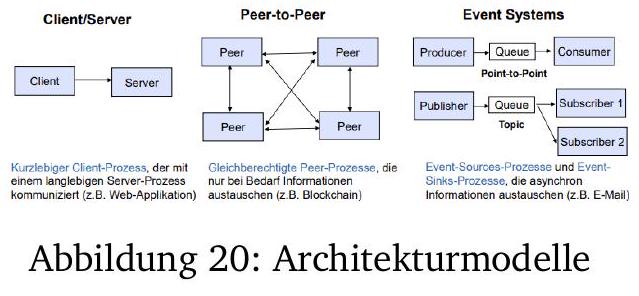
\includegraphics[max width=\textwidth, center]{2024_12_29_0d1d7b5551ea1b4b41bdg-18}

\subsection*{11.5 Gängige Technologien (Middleware) f. Informationssysteme und Internet-basierte Systeme}
Für die Entwicklung verteilter Systeme stehen verschiedene MiddlewareTechnologien zur Verfügung, die die Kommunikation und Integration von verteilten Komponenten erleichtern. Dazu gehören Messaging-Broker wie Apache

Kafka, Middleware-Frameworks wie CORBA (Common Object Request Broker Architecture) und RESTful Web Services.


	%\subsection{Common Pitfalls und Best Practices}

\begin{concept}{Common Pitfalls in JPA Implementation}
\textbf{N+1 Problem:}
\begin{itemize}
    \item \textbf{Symptom:} Für jedes Objekt wird eine zusätzliche Query ausgeführt
    \item \textbf{Lösung:} Join Fetch oder Eager Loading strategisch einsetzen
\end{itemize}

\textbf{LazyInitializationException:}
\begin{itemize}
    \item \textbf{Symptom:} Zugriff auf lazy geladene Referenz außerhalb der Session
    \item \textbf{Lösung:} Transaktionen korrekt abgrenzen
\end{itemize}

\textbf{Bidirektionale Beziehungen:}
\begin{itemize}
    \item \textbf{Symptom:} Inkonsistente Objektzustände
    \item \textbf{Lösung:} Helper-Methoden für Beziehungspflege
\end{itemize}
\end{concept}

\begin{KR}{Best Practices für Persistenz}
\textbf{1. Architektur-Ebene}
\begin{itemize}
    \item Repository für Datenzugriff
    \item Service für Geschäftslogik
    \item DTO für Datentransfer
\end{itemize}

\textbf{2. Entity Design}
\begin{itemize}
    \item Immutable wenn möglich
    \item Bean Validation nutzen
    \item Geschäftsregeln in Entity-Klassen
\end{itemize}

\textbf{3. Performance}
\begin{itemize}
    \item Caching Strategien
    \item Batch Processing
    \item Query Optimierung
\end{itemize}
\end{KR}

\subsection{Parent-Child Beziehungen}

\begin{concept}{Parent-Child Mapping}
\textbf{Implementationsaspekte:}
\begin{itemize}
    \item Cascade-Typen definieren
    \item Bidirektionale Navigation
    \item Lazy Loading konfigurieren
    \item Orphan Removal festlegen
\end{itemize}

\textbf{JPA Annotationen:}
\begin{itemize}
    \item @OneToMany / @ManyToOne
    \item @JoinColumn
    \item mappedBy Parameter
    \item fetch = FetchType.LAZY/EAGER
\end{itemize}
\end{concept}

\subsection{Repository Pattern}

\begin{concept}{Spring Data Repository}
\textbf{Vorteile:}
\begin{itemize}
    \item Standardisierte CRUD-Operationen
    \item Query-Methoden aus Methodennamen
    \item Paginierung und Sortierung
    \item Einfache Integration mit Spring
\end{itemize}

\textbf{Repository Hierarchie:}
\begin{itemize}
    \item Repository (Marker Interface)
    \item CrudRepository (Basis CRUD)
    \item PagingAndSortingRepository
    \item JpaRepository (JPA-spezifisch)
\end{itemize}
\end{concept}

\begin{KR}{Repository Design}
\textbf{1. Interface Definition}
\begin{itemize}
    \item Domänenspezifische Methoden
    \item Query-Methoden
    \item Custom Implementations
\end{itemize}

\textbf{2. Query Methoden}
\begin{itemize}
    \item Methodennamen-Konventionen
    \item @Query Annotation
    \item Native Queries
\end{itemize}

\textbf{3. Transaktionshandling}
\begin{itemize}
    \item @Transactional Annotation
    \item Isolation Level
    \item Propagation Rules
\end{itemize}
\end{KR}

\subsection{Performance Optimierung}

\begin{KR}{Optimierungsstrategien}
\textbf{1. Fetch-Strategien}
\begin{itemize}
    \item Lazy Loading als Default
    \item Joins für häufig benötigte Daten
    \item EntityGraphs für komplexe Szenarien
\end{itemize}

\textbf{2. Caching}
\begin{itemize}
    \item First-Level Cache (Session)
    \item Second-Level Cache
    \item Query Cache
\end{itemize}

\textbf{3. Batch-Verarbeitung}
\begin{itemize}
    \item Batch Inserts/Updates
    \item JDBC Batch Size
    \item Pagination für große Datensätze
\end{itemize}
\end{KR}

%todo: Add examples for:
% - Handling parent-child relationships
% - Repository implementation with Spring Data
% - Performance optimization scenarios
% - Common pitfall solutions

\begin{concept}{Transaktionsmanagement}
\textbf{ACID-Eigenschaften:}
\begin{itemize}
    \item Atomicity (Atomarität)
    \item Consistency (Konsistenz)
    \item Isolation (Isolation)
    \item Durability (Dauerhaftigkeit)
\end{itemize}

\textbf{Isolation Levels:}
\begin{itemize}
    \item READ\_UNCOMMITTED
    \item READ\_COMMITTED
    \item REPEATABLE\_READ
    \item SERIALIZABLE
\end{itemize}
\end{concept}
	%\section{Framework Design}

\begin{concept}{Framework Grundlagen}\\
Ein Framework ist ein Programmiergerüst mit folgenden Eigenschaften:
\begin{itemize}
    \item Bietet wiederverwendbare Funktionalität
    \item Definiert Erweiterungs- und Anpassungspunkte
    \item Verwendet Design Patterns
    \item Enthält keinen applikationsspezifischen Code
    \item Gibt Rahmen für anwendungsspezifischen Code vor
    \item Klassen arbeiten eng zusammen (vs. reine Bibliothek)
\end{itemize}
\end{concept}

\begin{definition}{Framework Entwicklung}\\
Die Entwicklung eines Frameworks erfordert:
\begin{itemize}
    \item Höhere Zuverlässigkeit als normale Software
    \item Tiefergehende Analyse der Erweiterungspunkte
    \item Hoher Architektur- und Designaufwand
    \item Sorgfältige Planung der Schnittstellen
\end{itemize}
\end{definition}

\begin{remark}{Kritische Betrachtung}\\
Herausforderungen beim Framework-Einsatz:
\begin{itemize}
    \item Frameworks tendieren zu wachsender Funktionalität
    \item Gefahr von inkonsistentem Design
    \item Funktionale Überschneidungen möglich
    \item Hoher Einarbeitungsaufwand
    \item Schwierige "Scheidung" nach Integration
    \item Trade-off zwischen Abhängigkeit und Nutzen
\end{itemize}
\end{remark}

\subsection{Design Patterns in Frameworks}

\begin{concept}{Abstract Factory}\\
\textbf{Problem:} Erzeugung verschiedener, zusammengehörender Objekte ohne Kenntnis konkreter Klassen\\
\textbf{Lösung:}
\begin{itemize}
    \item AbstractFactory-Interface definieren
    \item Pro Produkt eine create-Methode
    \item Konkrete Factories implementieren Interface
\end{itemize}
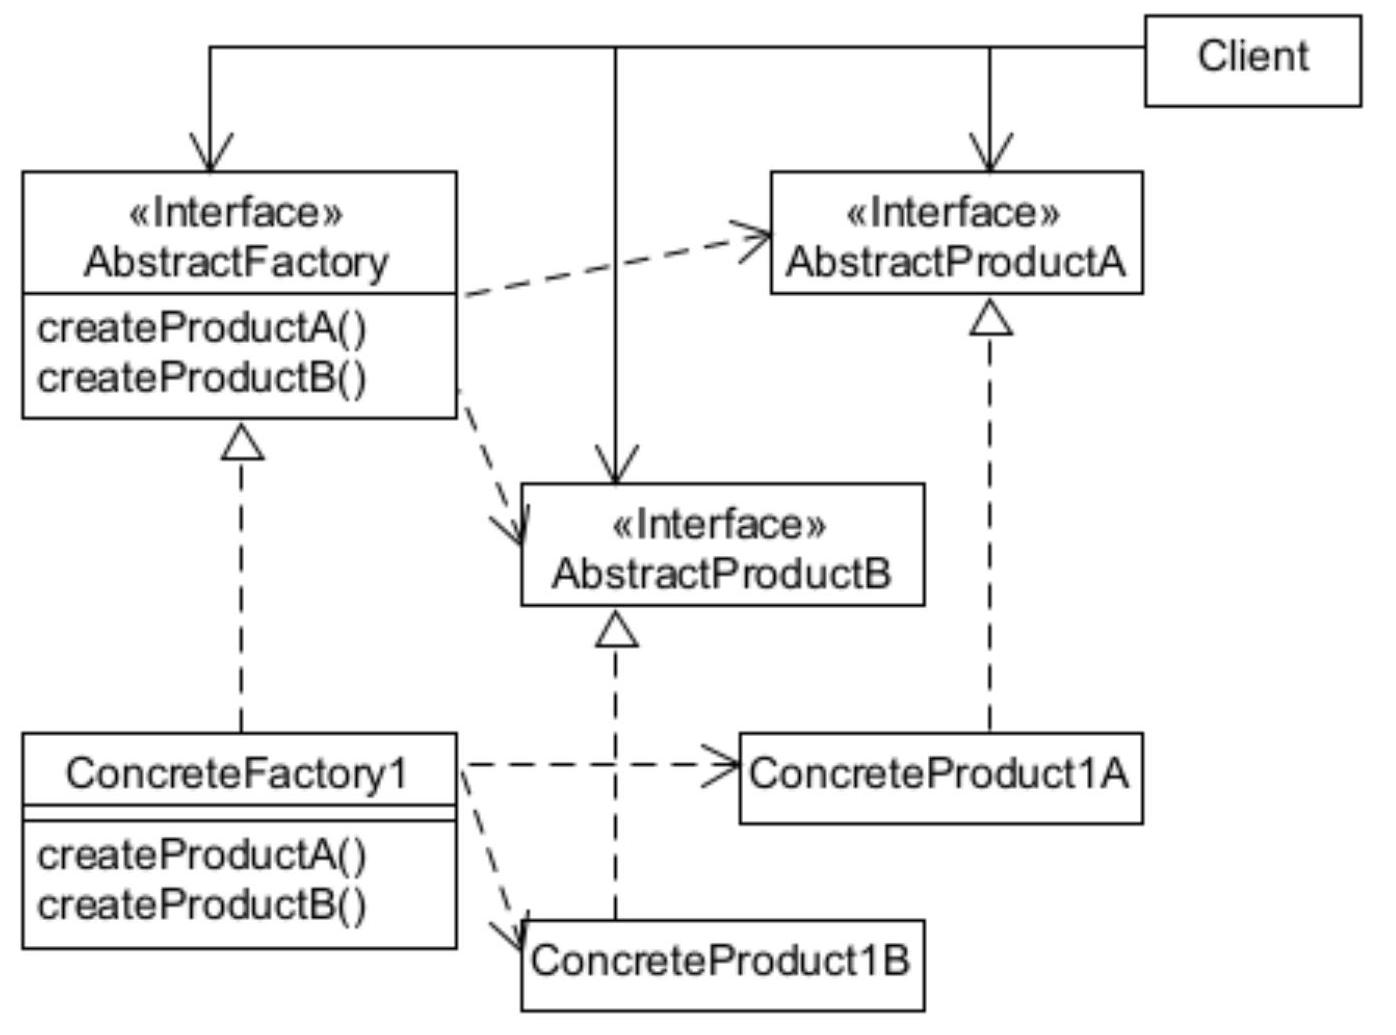
\includegraphics[width=0.8\linewidth]{images/2025_01_02_73d93f10fa91ab6123dcg-13}
\end{concept}

\begin{example}{Abstract Factory: POS Terminal}
\begin{lstlisting}[language=Java, style=base]
public interface IJavaPOSDevicesFactory {
    CashDrawer getNewCashDrawer();
    CoinDispenser getNewCoinDispenser();
    // weitere Methoden
}

public class IBMJavaPOSDevicesFactory 
        implements IJavaPOSDevicesFactory {
    public CashDrawer getNewCashDrawer() {
        return new com.ibm.pos.jpos.CashDrawer();
    }
    // weitere Implementierungen
}
\end{lstlisting}
\end{example}

\begin{concept}{Factory Method}\\
\textbf{Problem:} Flexible Objekterzeugung in wiederverwendbarer Klasse\\
\textbf{Lösung:}
\begin{itemize}
    \item Abstrakte Factory-Methode in Creator-Klasse
    \item Konkrete Subklassen überschreiben Methode
    \item Parallele Vererbungshierarchien
\end{itemize}
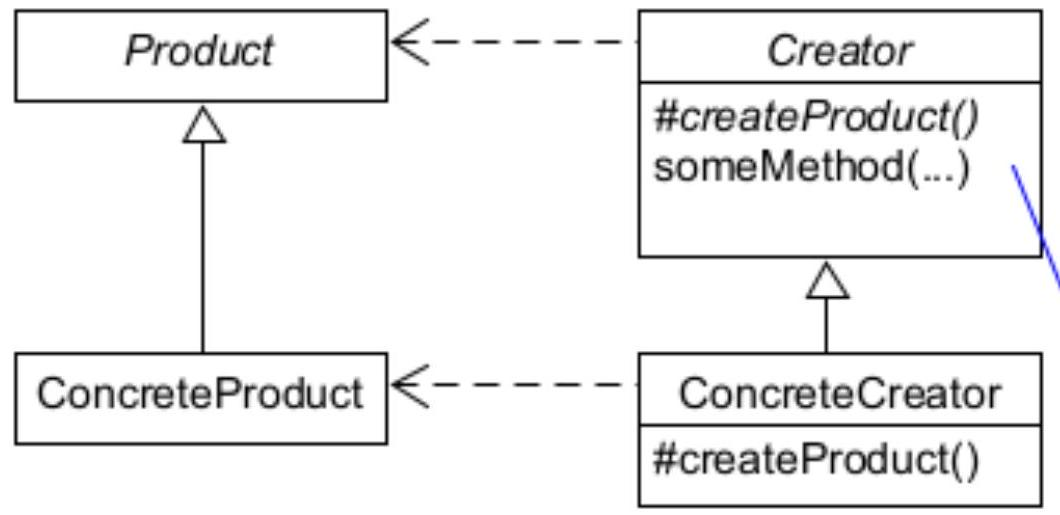
\includegraphics[width=0.8\linewidth]{images/2025_01_02_73d93f10fa91ab6123dcg-16}
\end{concept}

\begin{concept}{Command}\\
\textbf{Problem:} Aktionen für späteren Gebrauch speichern und verwalten\\
\textbf{Lösung:}
\begin{itemize}
    \item Command-Interface definieren
    \item Konkrete Commands implementieren
    \item Parameter für Ausführung speichern
    \item Optional: Undo-Funktionalität
\end{itemize}
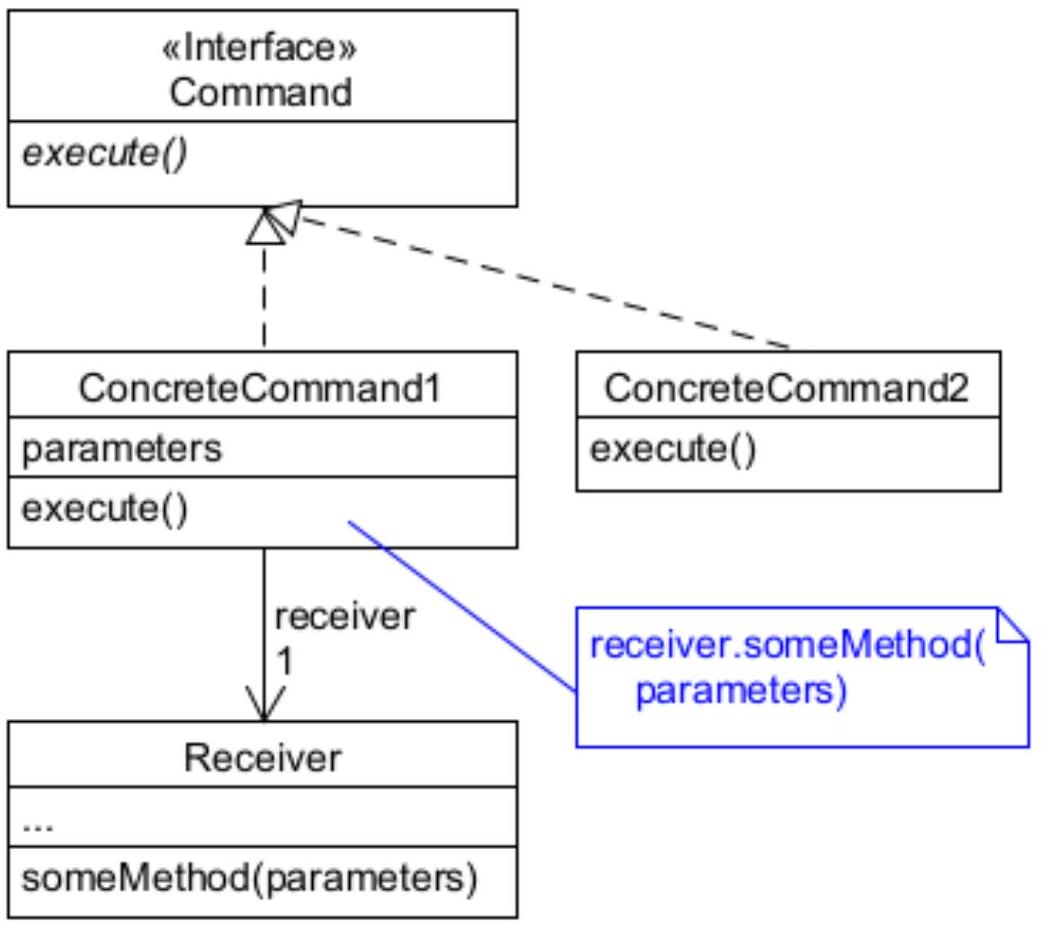
\includegraphics[width=0.8\linewidth]{images/2025_01_02_73d93f10fa91ab6123dcg-19}
\end{concept}

\begin{example}{Command: Persistenz}
\begin{lstlisting}[language=Java, style=base]
public interface ICommand {
    void execute();
    void undo();
}

public class DBUpdateCommand implements ICommand {
    private PersistentObject object;
    
    public void execute() {
        // Update in Datenbank
    }
    
    public void undo() {
        // Aenderung rueckgaengig machen
    }
}
\end{lstlisting}
\end{example}

\begin{concept}{Template Method}\\
\textbf{Problem:} Algorithmus mit anpassbaren Teilschritten\\
\textbf{Lösung:}
\begin{itemize}
    \item Template Method in abstrakter Klasse
    \item Hook-Methoden für variable Teile
    \item Hollywood Principle: "Don't call us, we'll call you"
\end{itemize}
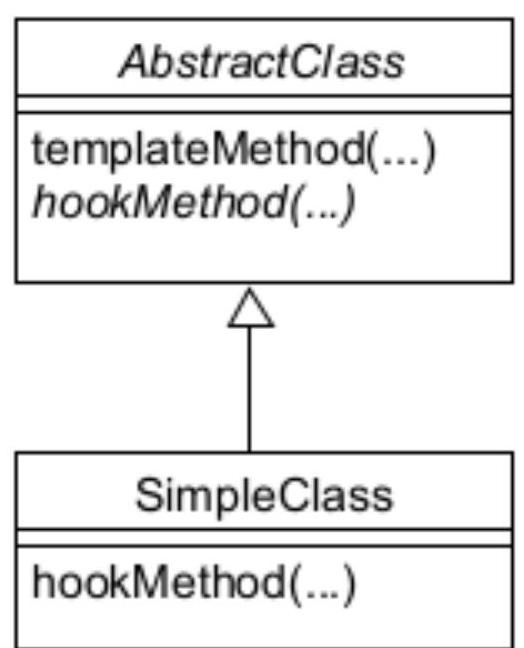
\includegraphics[width=0.8\linewidth]{images/2025_01_02_73d93f10fa91ab6123dcg-22}
\end{concept}

\begin{example}{Template Method: GUI Framework}
\begin{lstlisting}[language=Java, style=base]
public abstract class GUIComponent {
    // Template Method
    public final void update() {
        clearBackground();
        repaint(); // Hook Method
    }
    
    protected abstract void repaint();
}

public class MyButton extends GUIComponent {
    protected void repaint() {
        // Button-spezifische Implementation
    }
}
\end{lstlisting}
\end{example}

\subsection{Moderne Framework Patterns}

\begin{concept}{Annotation-basierte Konfiguration}\\
Moderne Frameworks nutzen Annotationen für:
\begin{itemize}
    \item Dependency Injection
    \item Konfiguration
    \item Interface-Implementation
    \item Funktionalitätserweiterung
\end{itemize}
\end{concept}

\begin{KR}{Framework Integration}
\begin{enumerate}
    \item \textbf{Convention over Configuration}
    \begin{itemize}
        \item Namenskonventionen einhalten
        \item Standard-Verhalten nutzen
        \item Nur Ausnahmen konfigurieren
    \end{itemize}
    
    \item \textbf{Dependency Injection}
    \begin{itemize}
        \item Abhängigkeiten deklarieren
        \item Framework übernimmt Injection
        \item Constructor- oder Setter-Injection
    \end{itemize}
    
    \item \textbf{Interface-basierte Entwicklung}
    \begin{itemize}
        \item Interfaces definieren
        \item Framework generiert Implementation
        \item Methodennamen als Spezifikation
    \end{itemize}
\end{enumerate}
\end{KR}

\begin{example}{Spring Data Repository}
\begin{lstlisting}[language=Java, style=base]
@Repository
public interface UserRepository 
        extends JpaRepository<User, Long> {
    // Methode wird automatisch implementiert
    List<User> findByLastNameOrderByFirstNameAsc(
        String lastName);
    
    // SQL-Query via Annotation
    @Query("SELECT u FROM User u WHERE u.active = true")
    List<User> findActiveUsers();
}
\end{lstlisting}
\end{example}

\begin{remark}
Annotation-basierte Frameworks bieten:
\begin{itemize}
    \item Geringere Kopplung zur Framework-API
    \item Deklarativen Programmierstil
    \item Reduzierte Boilerplate-Code
    \item Kann aber zu längeren Startzeiten führen
\end{itemize}
\end{remark}
	%\section{wrapup}

\section*{Angewendeter iterativ-inkrementeller Softwareentwicklungsprozess in SWEN1/PM3}
\begin{itemize}
  \item Der Softwareentwicklungsprozess wurde so angepasst (engl. tailoring), dass die wesentlichen Artefakte in einem Softwareprojekt im Kontext eingeführt werden können.
  \item Die Software wird in Iterationen entwickelt (2 Wochen Rhythmus).
  \item Jede Iteration hat ein Ziel und wird nach Abschluss reviewed.
  \item Es gibt drei Meilensteine, die im Projektverlauf ein besonderes Ereignis darstellen bzw. den Abschluss einer Phase: Projektskizze (M1), Lösungsarchitektur (M2) und Beta-Release (M3)
  \item In jeder Iteration werden Anforderungen, Analyse \& Design, Implementation und Testing gemacht (Software entsteht in Inkrementen).
  \item Der angewendete Softwareentwicklungsprozess und das Projektmanagement eines iterativ-inkrementellen Projektes wird in PM3 noch detaillierter erklärt.
\end{itemize}

\section*{Wesentliche Resultate bzw. Artefakte}
\begin{itemize}
  \item Anforderungsanalyse
  \item Funktionale Anforderungen mit Use Cases
  \item Qualitätsanforderungen und Randbedingungen
  \item Domänenmodell
  \item Design
  \item Softwarearchitektur
  \item Use Case Realisierung (statische und dynamische Modelle)
  \item Implementation
  \item Quellcode (inkl. Javadoc)
  \item Testing
  \item Unit-Tests\\
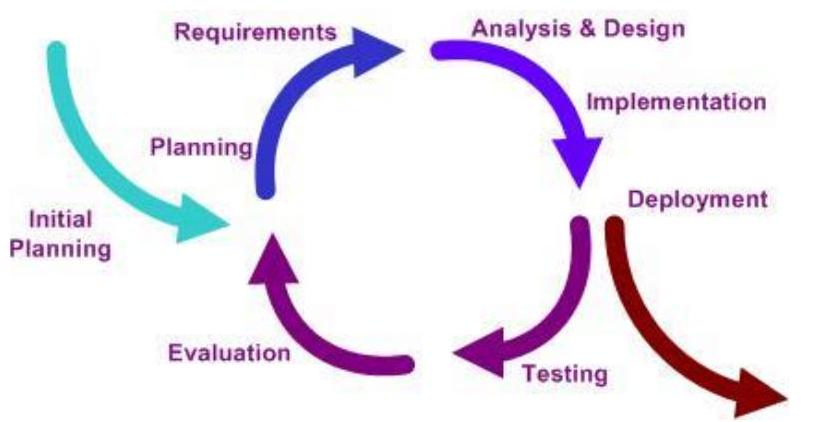
\includegraphics[max width=\textwidth, center]{2025_01_02_6eafa38dd4ae10c9a392g-09}
  \item Integrations- und Systemtests
\end{itemize}

\section*{Modellierung und Modelle mit der UML}

\includegraphics[max width=\textwidth, center]{2025_01_02_6eafa38dd4ae10c9a392g-10}\\
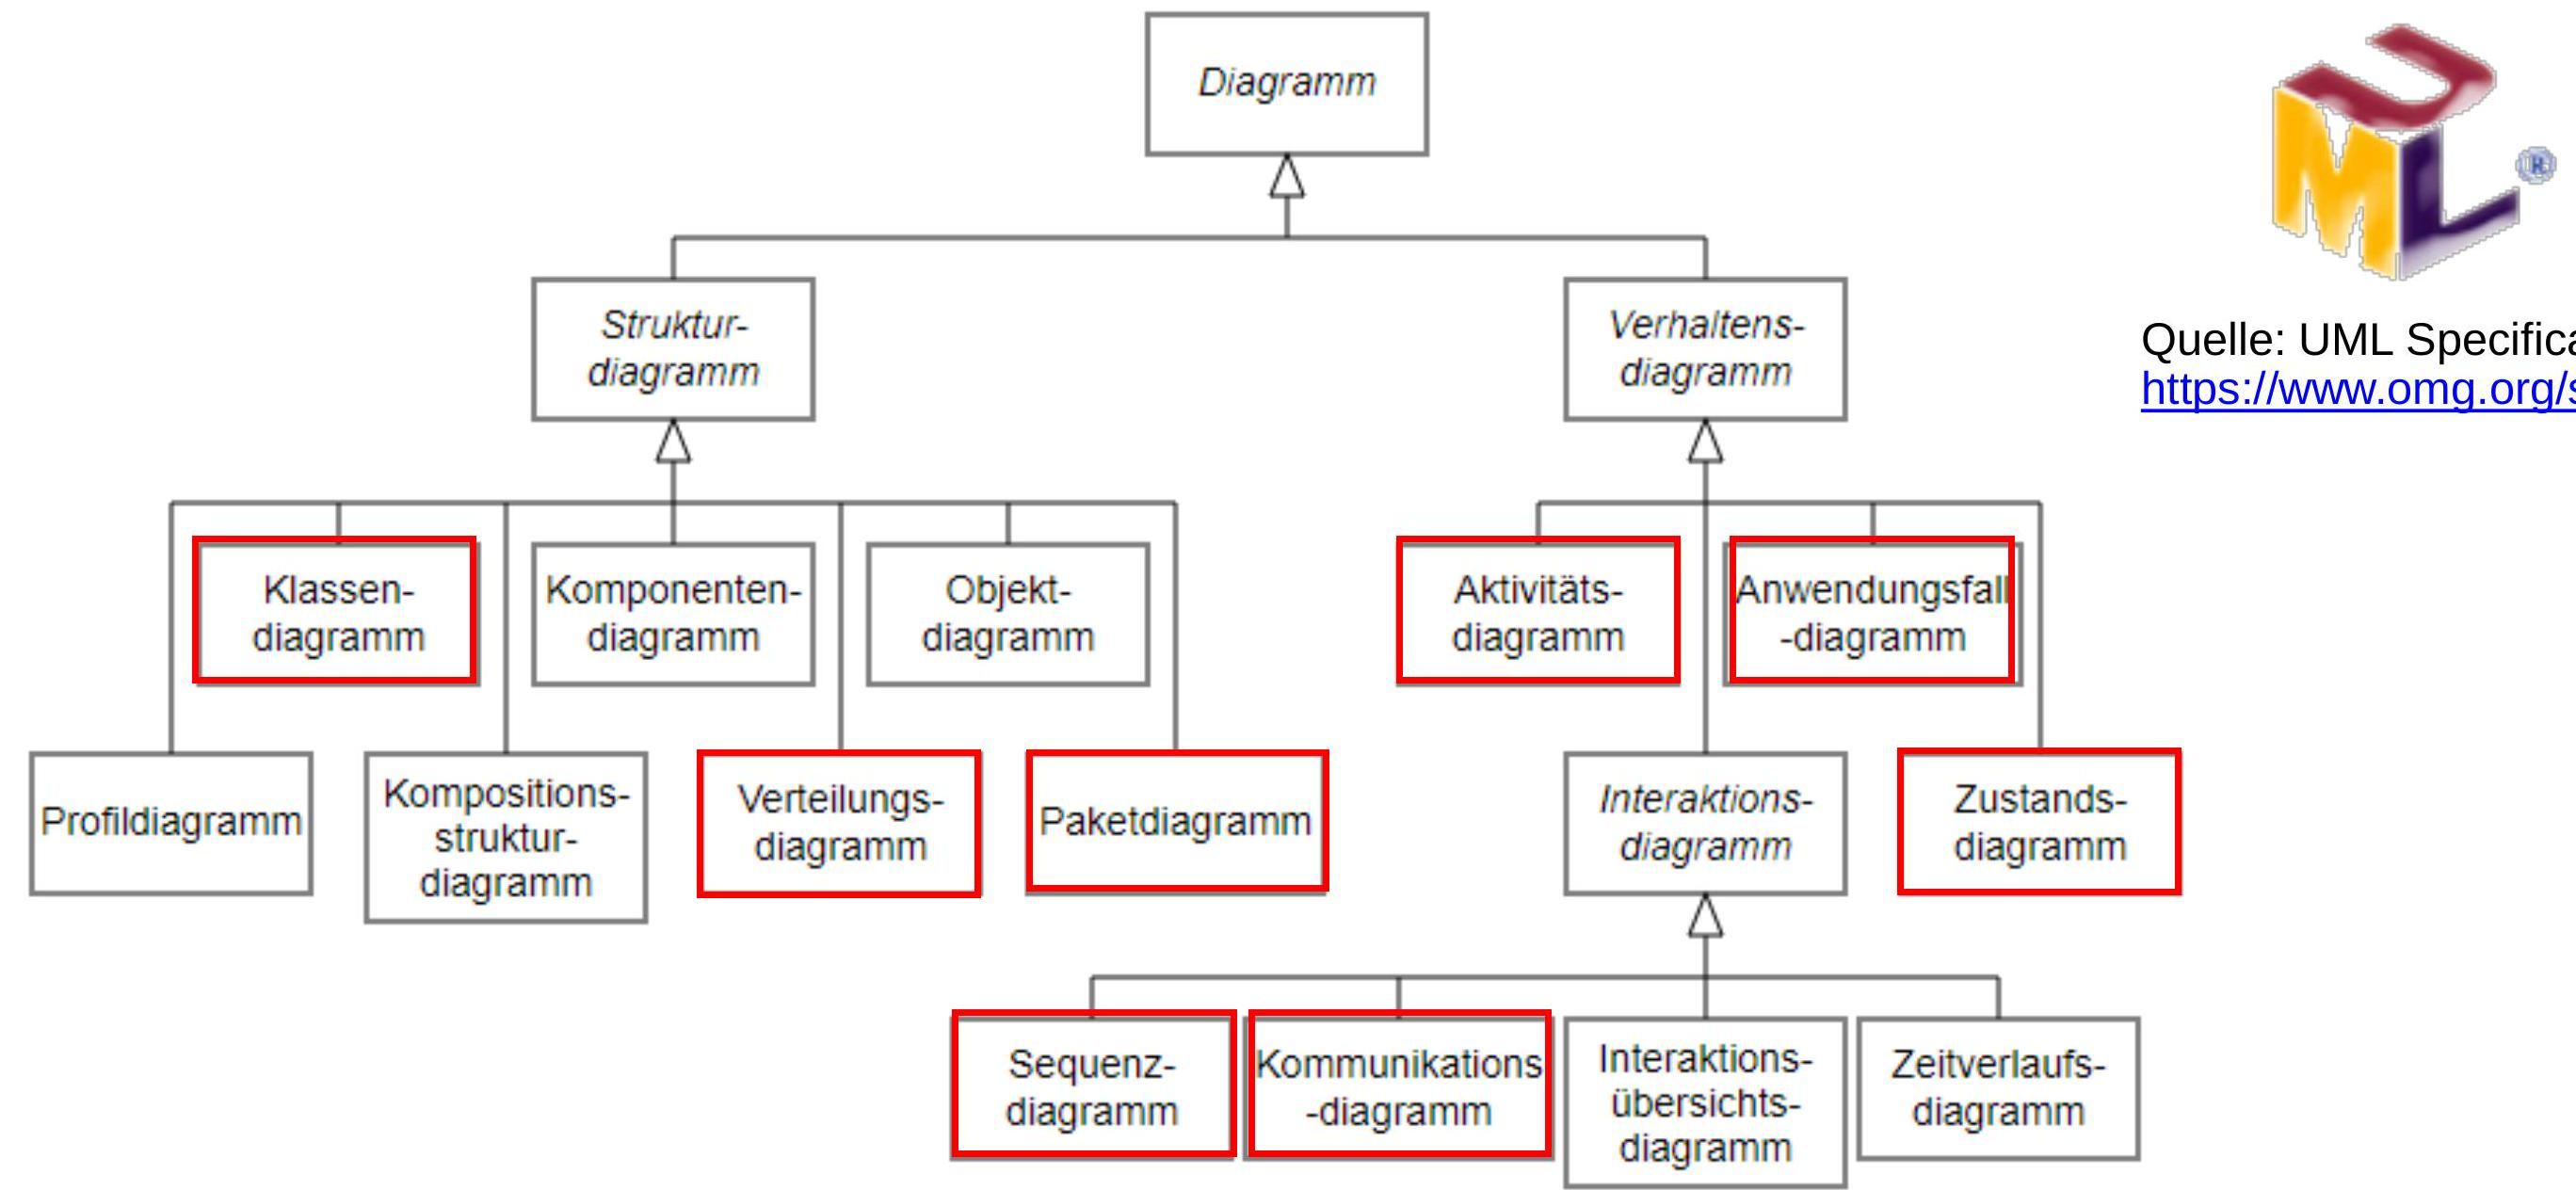
\includegraphics[max width=\textwidth, center]{2025_01_02_6eafa38dd4ae10c9a392g-10(1)}

Quelle: UML Specification, \href{https://www.omg.org/spec/UML/}{https://www.omg.org/spec/UML/}\\
$\square$ für die Modellierung in SWEN1 relevant

\section*{Gebrauch der UML (nach Martin Fowler)}
\section*{- UML as a Sketch}
\begin{itemize}
  \item Informelle und unvollständige Diagramme (z.T. von Hand gezeichnet), um schwierige Teile des Problems oder der Lösung zu verstehen und zu kommunizieren
  \item Die agile Community bevorzugt diese Anwendungsart von UML
  \item UML as a Blueprint
  \item Relativ detaillierte Analyse und Design-Diagramme für Code-Generierung oder um existierenden Code besser zu verstehen
  \item Klassische UML-Tools für ein Forward- und Reverse-Engineering (Roundtrip)
  \item UML as a Programming Language
  \item Komplete, ausführbare Spezifikation eines Software-Systems in UML
  \item MDA-Tools zur Modellierung und Generierung
\end{itemize}

\section*{Überblick Anforderungen \& Analyse}
\begin{itemize}
  \item User Research (Personas und Szenarien, Contextual Inquiry)
  \item Sketching und Protoyping
  \item Ableiten und Modellieren von Use Cases (dt. Anwendungsfälle)
  \item Detaillierung der Use Case (UML-Use-Case-Diagramm, Use-CaseSpezifikationen, UI-Sketching
  \item Qualitätsanforderungen und Randbedingungen erheben und festhalten.
  \item Modellierung der Fachlichkeit und Begriffe des Anwenders in einem Domänenmodell (konzeptuelles UML-Klassendiagramm)
  \item Bei der objektorientierten Analyse (OOA) liegt die Betonung darauf, die Objekte - oder Konzepte in dem Problembereich zu finden und zu beschreiben!
\end{itemize}

\section*{Überblick Design}
\begin{itemize}
  \item Design und Modellierung einer für die Problemstellung geeigneten Softwarearchitektur (UML-Paketdiagramm, UML-Verteilungsdiagramm)
  \item Use-Case-Realisierung und Klassendesign mit Verantwortlichkeiten (UML-Klassendiagramm, UML-Sequenzdiagramm, UMLKommunikationsdiagramm, UML-Zustandsdiagramm, UML-\\
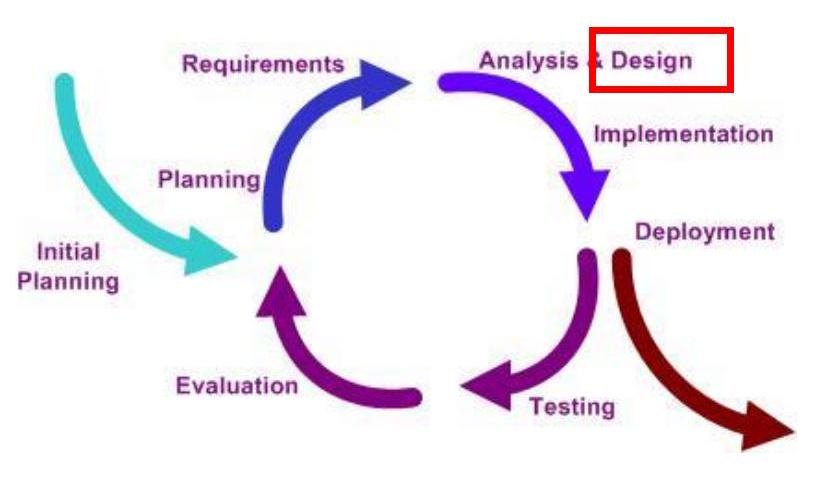
\includegraphics[max width=\textwidth]{2025_01_02_6eafa38dd4ae10c9a392g-13} Aktivitätsdiagramm)
  \item Entwurf mit bewährten Design Patterns
  \item Beim objektorientierten Design (OOD) liegt die Betonung darauf, geeignete Softwareobjekte und ihr Zusammenwirken (engl. collaboration) zu definieren, um die Anforderungen zu erfüllen!
\end{itemize}

\section*{Überblick Implementation}
\begin{itemize}
  \item Umsetzung des Designs in Code der entsprechenden (objektorientierten) Programmiersprache
  \item Verwendung von geeigneten Algorithmen und Datenstrukturen zur Implementierung des Designs
  \item Code Smells sofort bei deren Aufdeckung verbessern (Refactoring)\\
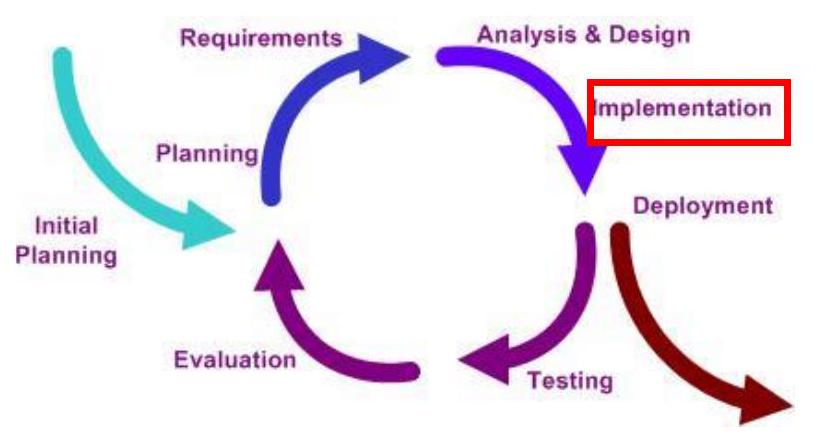
\includegraphics[max width=\textwidth, center]{2025_01_02_6eafa38dd4ae10c9a392g-14}
  \item Laufende Dokumentation des Quellcodes (nach Clean CodePrinzipien)
\end{itemize}

\section*{Überblick Testing}
\begin{itemize}
  \item Laufendes Design und Implementierung von Unit-Tests
  \item Planung, Design und Durchführung von weiteren Tests auf den Teststufen Integration und System je nach Problemstellung
  \item Dokumentation des Testkonzepts und der Tests\\
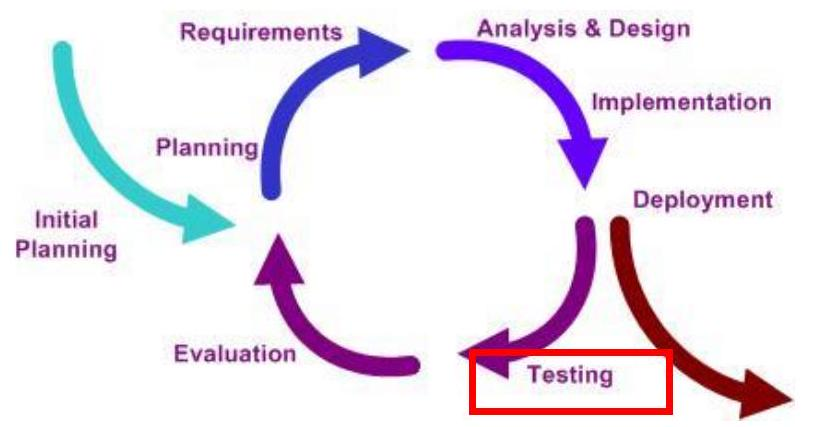
\includegraphics[max width=\textwidth, center]{2025_01_02_6eafa38dd4ae10c9a392g-15}
\end{itemize}
	\raggedcolumns
	\pagebreak
	\section{Additional Examples}

\subsection{Rechnerarithmetik}

\begin{example2}{Werteberechnung ausführlich} 
Gegeben sei die Maschinenzahl zur Basis $B=2$:
$$x = \underbrace{0.1101}_{\text{n=4}} \cdot \underbrace{2^{101}_2}_{\text{l=3}}$$

\textbf{1. Normalisierung prüfen:}
\begin{itemize}
    \item $m_1 = 1 \neq 0$ $\rightarrow$ normalisiert
\end{itemize}

\textbf{2. Exponent berechnen:}
\begin{align*}
\hat{e} &= 1 \cdot 2^2 + 0 \cdot 2^1 + 1 \cdot 2^0 \\
&= 4 + 0 + 1 = 5
\end{align*}

\textbf{3. Wert berechnen:}
\begin{align*}
\hat{\omega} &= 1 \cdot 2^{5-1} + 1 \cdot 2^{5-2} + 0 \cdot 2^{5-3} + 1 \cdot 2^{5-4} \\
&= 1 \cdot 2^4 + 1 \cdot 2^3 + 0 \cdot 2^2 + 1 \cdot 2^1 \\
&= 16 + 8 + 0 + 2 \\
&= 26
\end{align*}

Also ist $x = 26$
\end{example2}

\begin{example2}{Weitere Beispiele}
\begin{enumerate}
    \item Basis 10: $0.3141 \cdot 10^2$
    \begin{itemize}
        \item Normalisiert, da $m_1 = 3 \neq 0$
        \item $\hat{e} = 2$
        \item $\hat{\omega} = 3 \cdot 10^1 + 1 \cdot 10^0 + 4 \cdot 10^{-1} + 1 \cdot 10^{-2} = 31.41$
    \end{itemize}
    
    \item Basis 16 (hex): $0.A5F \cdot 16^3$
    \begin{itemize}
        \item Normalisiert, da $m_1 = A = 10 \neq 0$
        \item $\hat{e} = 3$
        \item $\hat{\omega} = 10 \cdot 16^2 + 5 \cdot 16^1 + 15 \cdot 16^0 = 2655$
    \end{itemize}
\end{enumerate}
\end{example2}

\begin{example2}{Werteberechnung} Berechnung einer Zahl zur Basis B=2:
\begin{minipage}{0.45\textwidth}
    $$\underbrace{0.1011}_{\text{n=4}} \cdot \underbrace{2^{3}}_{\text{l=1}}$$
\end{minipage}
\begin{minipage}[t]{0.5\textwidth}
    1. Exponent: $\hat{e} = 3$ \\ 
    2. Wert: $\hat{\omega} = 1\cdot2^2 + 0\cdot2^1 + 1\cdot2^0 + 1\cdot2^{-1}$ \\
    $= 4 + 0 + 1 + 0.5 = 5.5$
\end{minipage}
\end{example2}

\raggedcolumns


\subsection{Numerische Lösung von Nullstellenproblemen}

\begin{example2}{Fixpunktiteration} Nullstellen von $p(x)=x^3-x+0.3$\\
    %TODO: check if this is correct and/or relevant - either correct or replace with better example
Fixpunktgleichung: $x_{n+1} = F(x_n) = x_n^3 + 0.3$
\begin{enumerate}
    \item $F'(x) = 3x^2$ steigt monoton
    \item Für $I=[0,0.5]$: $F(0)=0.3 > 0$, $F(0.5)=0.425 < 0.5$
    \item $\alpha = \max_{x \in [0,0.5]} |3x^2| = 0.75 < 1$
    \item Konvergenz für Startwerte in $[0,0.5]$ gesichert
\end{enumerate}
\end{example2}



\begin{example2}{Newton-Verfahren} Berechnung von $\sqrt[3]{2}$
Nullstellenproblem: $f(x)=x^3-2$
\vspace{1mm}\\
\begin{minipage}[t]{0.65\textwidth}
    \vspace{-3mm}
    Ableitung: $f'(x)=3x^2$, Startwert $x_0=1$
    \begin{enumerate}
        \item $x_1 = 1 - \frac{1^3-2}{3 \cdot 1^2} = 1.333333$
        \item $x_2 = 1.333333 - \frac{1.333333^3-2}{3 \cdot 1.333333^2} = 1.259921$
        \item $x_3 = 1.259921 - \frac{1.259921^3-2}{3 \cdot 1.259921^2} = 1.259921$
    \end{enumerate}
\end{minipage}
\begin{minipage}[t]{0.3\textwidth}
    Quadratische Konvergenz sichtbar durch schnelle Annäherung an $\sqrt[3]{2} \approx 1.259921$
\end{minipage}
\end{example2}

\begin{example2}{Newton vs Sekanten}
Bestimmen Sie $\sqrt{2}$ mit beiden Verfahren.

\paragraph{Newton-Verfahren:} $f(x) = x^2-2$
\begin{itemize}
    \item $f'(x) = 2x$
    \item $x_0 = 1.5$
    \item $x_1 = 1.5 - \frac{1.5^2-2}{2\cdot1.5} = 1.4167$
    \item $x_2 = 1.4167 - \frac{1.4167^2-2}{2\cdot1.4167} = 1.4142$
\end{itemize}

\paragraph{Sekantenverfahren:}
\begin{itemize}
    \item $x_0 = 1$, $x_1 = 2$
    \item $x_2 = x_1 - \frac{x_1-x_0}{f(x_1)-f(x_0)}f(x_1) = 1.5$
    \item $x_3 = 1.5 - \frac{1.5-2}{1.5^2-2}1.5 = 1.4545$
    \item $x_4 = 1.4545 - \frac{1.4545-1.5}{1.4545^2-2}1.4545 = 1.4143$
\end{itemize}

\paragraph{Vergleich:}
\begin{itemize}
    \item Newton: Schnellere Konvergenz (quadratisch)
    \item Sekanten: Keine Ableitungsberechnung nötig
    \item Beide erreichen $10^{-4}$ Genauigkeit in 4-5 Schritten
\end{itemize}
\end{example2}

\subsection{Numerische Lösung von LGS}

\begin{example2}{Pivotisierung in der Praxis}
Betrachten Sie das System:
$$\begin{psmallmatrix}
0.001 & 1\\
1 & 1
\end{psmallmatrix}
\begin{psmallmatrix}
x_1\\
x_2
\end{psmallmatrix} = 
\begin{psmallmatrix}
1\\
2
\end{psmallmatrix}$$

\paragraph{Ohne Pivotisierung:}
Division durch 0.001 führt zu großen Rundungsfehlern:
$$x_1 \approx 1000 \cdot (1 - x_2)$$

\paragraph{Mit Pivotisierung:}
Nach Zeilenvertauschung:
$$\begin{psmallmatrix}
1 & 1\\
0.001 & 1
\end{psmallmatrix}
\begin{psmallmatrix}
x_1\\
x_2
\end{psmallmatrix} = 
\begin{psmallmatrix}
2\\
1
\end{psmallmatrix}$$
Liefert stabile Lösung: $x_1 = 1$, $x_2 = 1$
\end{example2}

\begin{example2}{Gauss mit Pivotisierung}
Lösen Sie $Ax = b$ mit:
$$A = \begin{pmatrix} 
1 & 2 & 1 \\
2 & 4 & -1 \\
4 & -2 & 1
\end{pmatrix}, \quad b = \begin{pmatrix} 1 \\ 2 \\ 0 \end{pmatrix}$$

\paragraph{Lösung:}
\begin{enumerate}
    \item Erste Spalte: Pivot $a_{31} = 4$ $\rightarrow$ Z1 $\leftrightarrow $ Z3
    $$\begin{pmatrix} 
    4 & -2 & 1 & | & 0 \\
    2 & 4 & -1 & | & 2 \\
    1 & 2 & 1 & | & 1
    \end{pmatrix}$$
    
    \item Eliminationsschritte:
    $$\begin{pmatrix} 
    4 & -2 & 1 & | & 0 \\
    0 & 5 & -1.5 & | & 2 \\
    0 & 2.5 & 0.75 & | & 1
    \end{pmatrix}$$
    $$\begin{pmatrix} 
    4 & -2 & 1 & | & 0 \\
    0 & 5 & -1.5 & | & 2 \\
    0 & 0 & 1.5 & | & 0.2
    \end{pmatrix}$$
    
    \item Rückwärtseinsetzen:
    \begin{align*}
        x_3 &= 0.2/1.5 = \frac{2}{15} \\
        x_2 &= (2 + 1.5 \cdot \frac{2}{15})/5 = 0.5 \\
        x_1 &= (0 + 2 \cdot 0.5 - 1 \cdot \frac{2}{15})/4 = 0.2
    \end{align*}
\end{enumerate}
\end{example2}

\begin{example2}{LR-Zerlegung mit Pivotisierung}
Gegeben sei das System:
$$A = \begin{psmallmatrix}
1 & 2 & 1\\
3 & 8 & 1\\
0 & 4 & 1
\end{psmallmatrix}, \quad b = \begin{psmallmatrix}
2\\
3\\
5
\end{psmallmatrix}$$

\paragraph{1. Erste Spalte}
Max Element in 1. Spalte: $|a_{21}| = 3$, tausche Z1 und Z2:
$$P_1 = \begin{psmallmatrix}
0 & 1 & 0\\
1 & 0 & 0\\
0 & 0 & 1
\end{psmallmatrix}, \quad 
A^{(1)} = \begin{psmallmatrix}
3 & 8 & 1\\
1 & 2 & 1\\
0 & 4 & 1
\end{psmallmatrix}$$

Eliminationsfaktoren: $l_{21} = \frac{1}{3}$, $l_{31} = 0$\\
Nach Elimination:
$$A^{(2)} = \begin{psmallmatrix}
3 & 8 & 1\\
0 & -\frac{2}{3} & \frac{2}{3}\\
0 & 4 & 1
\end{psmallmatrix}$$

\paragraph{2. Zweite Spalte}
Max Element: $|a_{32}| = 4$, tausche Z2 und Z3:
$$P_2 = \begin{psmallmatrix}
1 & 0 & 0\\
0 & 0 & 1\\
0 & 1 & 0
\end{psmallmatrix}$$

Eliminationsfaktor: $l_{32} = -\frac{1}{6}$\\
Nach Elimination:
$$R = \begin{psmallmatrix}
3 & 8 & 1\\
0 & 4 & 1\\
0 & 0 & \frac{5}{6}
\end{psmallmatrix}$$

\paragraph{Endergebnis}
$$P = P_2P_1 = \begin{psmallmatrix}
0 & 1 & 0\\
0 & 0 & 1\\
1 & 0 & 0
\end{psmallmatrix}, \quad
L = \begin{psmallmatrix}
1 & 0 & 0\\
\frac{1}{3} & 1 & 0\\
0 & -\frac{1}{6} & 1
\end{psmallmatrix}$$

\paragraph{Lösung des Systems}
\begin{enumerate}
    \item $Pb = \begin{psmallmatrix} 3\\ 5\\ 2 \end{psmallmatrix}$
    \item $Ly = Pb$: $y = \begin{psmallmatrix} 3\\ 4\\ 1 \end{psmallmatrix}$
    \item $Rx = y$: $x = \begin{psmallmatrix} 1\\ 0\\ \frac{6}{5} \end{psmallmatrix}$
\end{enumerate}
\end{example2}

\begin{KR}{Umgang mit Systemen mit freien Variablen}
\begin{enumerate}
    \item Vorgehensweise
    \begin{itemize}
        \item Matrix auf Stufenform bringen
        \item Freie Variablen identifizieren (Nullspalten)
        \item Basislösung berechnen
        \item Allgemeine Lösung parametrisch aufstellen
    \end{itemize}
    
    \item Interpretation
    \begin{itemize}
        \item Rang der Matrix bestimmen
        \item Lösbarkeit prüfen
        \item Dimension des Lösungsraums bestimmen
        \item Spezielle Lösungen generieren
    \end{itemize}
    
    \item Sonderfälle beachten
    \begin{itemize}
        \item Unlösbare Systeme erkennen
        \item Abhängige Gleichungen identifizieren
        \item Numerische Genauigkeit berücksichtigen
    \end{itemize}
\end{enumerate}
\end{KR}

\begin{example2}{QR-Zerlegung}
Gegeben sei die Matrix:
$$A = \begin{psmallmatrix}
1 & 1\\
1 & 0\\
0 & 1
\end{psmallmatrix}$$

\paragraph{1. Erste Spalte}
$v_1 = \begin{psmallmatrix} 1\\ 1\\ 0 \end{psmallmatrix}$, 
$\|v_1\| = \sqrt{2}$

Householder-Vektor:
$w_1 = v_1 + \sqrt{2}\begin{psmallmatrix} 1\\ 0\\ 0 \end{psmallmatrix} = 
\begin{psmallmatrix} 1+\sqrt{2}\\ 1\\ 0 \end{psmallmatrix}$

Normierung:
$u_1 = \frac{1}{\sqrt{4+2\sqrt{2}}}
\begin{psmallmatrix} 1+\sqrt{2}\\ 1\\ 0 \end{psmallmatrix}$

Erste Householder-Matrix:
$$H_1 = I - 2u_1u_1^T = 
\begin{psmallmatrix}
-\frac{1}{\sqrt{2}} & -\frac{1}{\sqrt{2}} & 0\\
-\frac{1}{\sqrt{2}} & \frac{1}{\sqrt{2}} & 0\\
0 & 0 & 1
\end{psmallmatrix}$$

\paragraph{2. Zweite Spalte}
Nach Anwendung von $H_1$:
$$H_1A = \begin{psmallmatrix}
-\sqrt{2} & -\frac{1}{\sqrt{2}}\\
0 & \frac{1}{\sqrt{2}}\\
0 & 1
\end{psmallmatrix}$$

Untervektor für zweite Transformation:
$v_2 = \begin{psmallmatrix} \frac{1}{\sqrt{2}}\\ 1 \end{psmallmatrix}$

Analog zur ersten Transformation erhält man:
$$H_2 = \begin{psmallmatrix}
1 & 0 & 0\\
0 & -\frac{1}{\sqrt{5}} & -\frac{2}{\sqrt{5}}\\
0 & -\frac{2}{\sqrt{5}} & \frac{1}{\sqrt{5}}
\end{psmallmatrix}$$

\paragraph{Endergebnis}
$$Q = H_1^TH_2^T = \begin{psmallmatrix}
\frac{1}{\sqrt{2}} & \frac{1}{\sqrt{2}} & 0\\
\frac{1}{\sqrt{2}} & -\frac{1}{\sqrt{2}} & 0\\
0 & 0 & 1
\end{psmallmatrix}$$

$$R = H_2H_1A = \begin{psmallmatrix}
\sqrt{2} & 1\\
0 & \sqrt{2}\\
0 & 0
\end{psmallmatrix}$$

\paragraph{Verifikation}
\begin{itemize}
    \item $Q^TQ = QQ^T = I$ (Orthogonalität)
    \item $QR = A$ (bis auf Rundungsfehler)
    \item R ist obere Dreiecksmatrix
\end{itemize}
\end{example2}

\begin{example2}{Iterative Verfahren}{Vergleich Jacobi und Gauss-Seidel}
System:
$$\begin{psmallmatrix}
4 & -1 & 0\\
-1 & 4 & -1\\
0 & -1 & 4
\end{psmallmatrix}x = \begin{psmallmatrix}
1\\
5\\
0
\end{psmallmatrix}$$

\begin{center}
\begin{tabular}{c|cc|cc}
k & \multicolumn{2}{c|}{Jacobi} & \multicolumn{2}{c}{Gauss-Seidel}\\
\hline
0 & $(0,0,0)^T$ & & $(0,0,0)^T$ &\\
1 & $(0.25,1.25,0)^T$ & 1.25 & $(0.25,1.31,0.08)^T$ & 1.31\\
2 & $(0.31,1.31,0.31)^T$ & 0.31 & $(0.33,1.33,0.33)^T$ & 0.02\\
3 & $(0.33,1.33,0.33)^T$ & 0.02 & $(0.33,1.33,0.33)^T$ & 0.00
\end{tabular}
\end{center}
\end{example2}




\subsection{Eigenvektoren und Eigenwerte}

\begin{example2}{Darstellungsformen}
Gegeben: $z = 3 - 11i$ in Normalform
$$r = \sqrt{3^2 + 11^2} = \sqrt{130}, \quad \varphi = \arcsin(\frac{11}{\sqrt{130}}) = 1.3 \text{rad} = 74.74^{\circ}$$
\textbf{Trigonometrische Form:} $z = \sqrt{130}(\cos(1.3) + i\sin(1.3))$
\vspace{2mm}\\
\textbf{Exponentialform:} $z = \sqrt{130}e^{i\cdot 1.3}$
\end{example2}

\begin{example2}{Eigenwertberechnung}
%TODO: check if this is correct and/or relevant - either correct or replace with better example
$A = \begin{psmallmatrix} 1 & 0 & 0\\ 2 & 3 & 0\\ 0 & 1 & 2\end{psmallmatrix}$
\begin{enumerate}
    \item Da $A$ eine Dreiecksmatrix ist, sind die Diagonalelemente die \\
    Eigenwerte:
    $\lambda_1 = 1, \lambda_2 = 3, \lambda_3 = 2$
    \item $\det(A) = \lambda_1\cdot\lambda_2\cdot\lambda_3 = 6$
    \item $\operatorname{tr}(A) = \lambda_1 + \lambda_2 + \lambda_3 = 6$
    \item Spektrum: $\sigma(A) = \{1,2,3\}$
\end{enumerate}
\end{example2}

\begin{example2}{Von-Mises-Iteration}
Berechne größten Eigenwert der Matrix:
\vspace{2mm}\\
$A = \begin{psmallmatrix}
4 & -1 & 1\\
-1 & 3 & -2\\
1 & -2 & 3
\end{psmallmatrix}$, $\quad$
Startvektor: $v^{(0)} = \begin{psmallmatrix}1\\ 0\\ 0\end{psmallmatrix}$

\begin{center}
\begin{tabular}{c|c|c}
k & $v^{(k)}$ & $\lambda^{(k)}$ \\\hline
0 & $(1, 0, 0)^T$ & -\\
1 & $(0.970, -0.213, 0.119)^T$ & 4.000\\
2 & $(0.957, -0.239, 0.164)^T$ & 4.827\\
3 & $(0.953, -0.244, 0.178)^T$ & 4.953\\
4 & $(0.952, -0.245, 0.182)^T$ & 4.989
\end{tabular}
\end{center}

Konvergenz gegen $\lambda_1 \approx 5$ \\ Eigenvektor $v \approx (0.952, -0.245, 0.182)^T$
\end{example2}

\begin{example2}{Von-Mises-Iteration}
Bestimmen Sie den betragsmäßig größten Eigenwert von:
$$A = \begin{psmallmatrix}
3 & 1 \\
1 & 3
\end{psmallmatrix}$$

\paragraph{Lösung:}
\begin{enumerate}
    \item Start mit $v^{(0)} = \frac{1}{\sqrt{2}}\begin{psmallmatrix} 1 \\ 1 \end{psmallmatrix}$
    
    \item Erste Iteration:
    \begin{itemize}
        \item $w^{(0)} = \begin{psmallmatrix} 4 \\ 4 \end{psmallmatrix}$
        \item $v^{(1)} = \frac{1}{\sqrt{2}}\begin{psmallmatrix} 1 \\ 1 \end{psmallmatrix}$
        \item $\lambda^{(1)} = 4$
    \end{itemize}
    
    \item Ergebnis:
    \begin{itemize}
        \item Eigenvektor bereits gefunden
        \item Eigenwert $\lambda = 4$ ist korrekt
    \end{itemize}
\end{enumerate}
\end{example2}

\begin{example2}{QR-Verfahren}
Matrix:
$$A = \begin{psmallmatrix}
2 & -1 & 1\\
-1 & 3 & 0\\
1 & 0 & 1
\end{psmallmatrix}$$

\paragraph{QR-Iteration:}
\begin{enumerate}
    \item $A_0 = A$
    \item Nach erster Iteration:
    $$A_1 = \begin{psmallmatrix}
    3.21 & -0.83 & 0.62\\
    -0.83 & 2.13 & 0.41\\
    0.62 & 0.41 & 0.66
    \end{psmallmatrix}$$
    \item Nach 5 Iterationen:
    $$A_5 \approx \begin{psmallmatrix}
    4 & 0 & 0\\
    0 & 1 & 0\\
    0 & 0 & 1
    \end{psmallmatrix}$$
\end{enumerate}

Die Diagonalelemente von $A_5$ sind die Eigenwerte: $\lambda_1 = 4, \lambda_2 = 1, \lambda_3 = 1$
\end{example2}
	\raggedcolumns
\end{multicols}
\end{document}
